%%% The main file. It contains definitions of basic parameters and includes all other parts.

%% Settings for single-side (simplex) printing
% Margins: left 40mm, right 25mm, top and bottom 25mm
% (but beware, LaTeX adds 1in implicitly)
\documentclass[12pt,notitlepage,a4paper,openright]{report}
\pagestyle{plain}
\usepackage{url}
\def\UrlBreaks{\do\/\do-}
\PassOptionsToPackage{hyperfootnotes=false}{hyperref}

% fix pdfx
\usepackage{etoolbox}
% \makeatletter
% \@ifl@t@r\fmtversion{2021-06-01}%
%  {\AddToHook{package/after/xmpincl}
%    {\patchcmd\mcs@xmpincl@patchFile{\if\par}{\ifx\par}{}{\fail}}}{}
% \makeatother

\usepackage[usenames,dvipsnames,svgnames,table,rgb]{xcolor}
\usepackage[a-2u]{pdfx}
\usepackage{fontspec}
\usepackage[czech,english]{babel}
\usepackage{lmodern}
\usepackage{textcomp}
\usepackage[defaultlines=4,all]{nowidow}

% Turn this on when needed:
\usepackage{microtype}

\usepackage{graphicx}
\usepackage[twoside, inner=3.7cm, outer=2.9cm, top=2.6cm, bottom=3.4cm]{geometry}
\usepackage{thesis}
\usepackage[round]{natbib}
\usepackage{multirow}
\usepackage{arydshln} % dashed lines in tables
\usepackage{array}
\usepackage{amssymb,latexsym,pifont}
\usepackage{amsmath}
\usepackage{enumitem} % custom lists
\usepackage[normalem]{ulem} % underlining
\usepackage{setspace} % line spacing
\usepackage{varioref} % nice references (above/below)
\usepackage[above,section]{placeins} % avoid figures pushed at end of chapters
\usepackage{listings}

\setlist[itemize]{itemsep=0.02cm,topsep=0.2cm}
\setlist[enumerate]{itemsep=0.02cm,topsep=0.2cm,label={(\arabic*)}}

\usepackage{tabularx}
\usepackage{booktabs} % nicer lines in table
\usepackage{multicol}
\usepackage{tikz}
\usepackage{pgfplots}
\pgfplotsset{compat=1.17}
\usepackage{gnuplot-lua-tikz}
\usetikzlibrary{shapes.geometric}
\usepackage{epstopdf}
\usepackage{algorithmicx}
\usepackage{algorithm}
\usepackage{algpseudocode}
\usepackage{mathtools}
\usepackage{quoting,xparse}
\usepackage{tikz}
\usepackage{cleveref}
% oxford comma
\newcommand{\creflastconjunction}{, and\nobreakspace}

% \usepackage[parfill]{parskip}

% acronyms and glossaries
\usepackage[acronym, nomain]{glossaries}
\usepackage[shortcuts=ac]{glossaries-extra}
\makeglossaries
\preto\chapter{\glsresetall}

\setabbreviationstyle[acronym]{long-short}

\usepackage{subcaption} % sub figures in a fiture
\usepackage{standalone} % include standoalone tikz images
\usepackage{bibentry}

\def\ZK#1{{\color{green!60!black!100}ZK: \it #1}}
\def\ZKdel#1{{\color{green!60!black!100}ZKdel: {\sout{#1}}}}
\def\TODO#1{{\color{green!60!black!100}TODO: \it #1}}

% hack bibentry command for list of publications
\makeatletter
\renewcommand\bibentry[1]{\nocite{#1}{\frenchspacing
     \@nameuse{BR@r@#1\@extra@b@citeb}}}
\makeatother

\renewcommand{\chapterautorefname}{Chapter}
\renewcommand{\sectionautorefname}{Section}
\renewcommand{\subsectionautorefname}{Section}
\renewcommand{\subsubsectionautorefname}{Section}



\definecolor{mydarkblue}{rgb}{0,0.08,0.45}
\hypersetup{ %
  colorlinks=true,
  linkcolor=black,
  citecolor=mydarkblue,
  filecolor=mydarkblue,
  urlcolor=mydarkblue,
  unicode=true
}

% \hypersetup{
%     colorlinks=false,
%     pdfborder={0 0 0},
%     unicode=true,
% }

\newcommand*\myglsentry[1]{%
  \protect\ifglsused{#1}{%
    \glsentryshort{#1}%
  }{%
    \glsentrylong{#1}%
  }%
}


%\newacronym{ai}{AI}{artificial intelligence}
%\newacronym{agi}{AGI}{artificial general intelligence}
%\newacronym{ar}{AR}{autoregressive}
%\newacronym{bleu}{BLEU}{bilingual evaluation understudy}
%\newacronym{bow}{BoW}{bag of words}
%\newacronym{bpe}{BPE}{byte-pair encoding}
%\newacronym{bptt}{BPTT}{backpropagation through time}
%\newacronym{ce}{CE}{cross-entropy}
%\newacronym{cf}{CF}{catastrophic forgetting}
%\newacronym{ci}{CI}{catastrophic interference}
%\newacronym{cifar}{CIFAR-10}{Canadian Institute For Advanced Research}
%\newacronym{cnn}{CNN}{convolutional neural network}
%\newacronym{comet}{COMET}{Crosslingual Optimized Metric for Evaluation of Translation}
%\newacronym{dan}{DAN}{deep averaging network}
%\newacronym{dl}{DL}{deep learning}
%\newacronym{elbo}{ELBO}{evidence lower bound}
%\newacronym{em}{EM}{expectation-maximization}
%\newacronym{eos}{EOS}{end-of-sequence}
%\newacronym{ewc}{EWC}{elastic weight consolidation}
%\newacronym{ffn}{FFN}{feed-forward network}
%\newacronym{fi}{FI}{Fisher information}
%\newacronym{fim}{FIM}{Fisher information matrix}
%\newacronym{glue}{GLUE}{General Language Understanding Evaluation}
%\newacronym{gru}{GRU}{gated recurrent unit}
%\newacronym{hmm}{HMM}{hidden Markov model}
%\newacronym{idf}{IDF}{inverse document frequency}
%\newacronym{iid}{IID}{independent and identically distributed}
%\newacronym{il}{IL}{incremental learning}
%\newacronym{iwslt}{IWSLT}{International Conference on Spoken Language Translation}
%\newacronym{kl}{KL}{Kullback–Leibler}
%\newacronym{ldd}{LDD}{long-distance dependencies}
%\newacronym{lm}{LM}{language model}
%\newacronym{lstm}{LSTM}{long short-term Memory}
%\newacronym{map}{MAP}{maximum a posteriori}
%\newacronym{mee}{MEE}{maximum entropy estimation}
%\newacronym{mffn}{MFFN}{masked feed-forward network}
%\newacronym{mha}{MHA}{multi-head attention}
%\newacronym{mmha}{MMHA}{masked multi-head attention}
%\newacronym{ml}{ML}{machine learning}
%\newacronym{mlm}{MLM}{masked language model}
%\newacronym{mlp}{MLP}{multi-layered perceptron}
%\newacronym{mmt}{MMT}{multimodal machine translation}
%\newacronym{mnist}{MNIST}{Modified National Institute of Standards and Technology}
%\newacronym{mrt}{MRT}{minimum risk training}
%\newacronym{mscoco}{MSCOCO}{Microsoft Common Objects in Context}
\newacronym{mt}{MT}{machine translation}
%\newacronym{mtl}{MTL}{multi-task learning}
%\newacronym{nar}{NAR}{non-autoregressive}
%\newacronym{nli}{NLI}{natural language inference}
%\newacronym{nll}{NLL}{negative log-likelihood}
\newacronym{nlp}{NLP}{natural language processing}
%\newacronym{moe}{MoE}{mixture-of-experts}
\newacronym{nmt}{NMT}{neural machine translation}
%\newacronym{nn}{NN}{neural network}
%\newacronym{oov}{OOV}{out-of-vocabulary}
\newacronym{pbmt}{PBMT}{phrase-based machine translation}
%\newacronym{pi}{PI}{path integral}
%\newacronym{qa}{QA}{question answering}
%\newacronym{rbf}{RBF}{radial basis function}
%\newacronym{relu}{ReLU}{rectified linear unit}
%\newacronym{rl}{RL}{reinforcement learning}
%\newacronym{rouge}{ROUGE}{Recall-Oriented Understudy for Gisting Evaluation}
%\newacronym{rnn}{RNN}{recurrent neural network}
%\newacronym{sgd}{SGD}{stochastic gradient descent}
%\newacronym{smt}{SMT}{statistical machine translation}
%\newacronym{sota}{SoTA}{state-of-the-art}
%\newacronym{squad}{SQuAD}{Stanford Question Answering Dataset}
%\newacronym{ste}{STE}{straight-through estimator}
%\newacronym{ted}{TED}{Technology, Entertainment and Design}
%\newacronym{ter}{TER}{Translation Error Rate}
%\newacronym{tfidf}{TF-IDF}{term frequency-inverse document frequency}
%\newacronym{wmt}{WMT}{Conference on Machine Translation}

%\newacronym{wngt}{WNGT}{Workshop on Neural Generation and Translation}
%\newacronym{xlm}{XLM}{cross-lingual language model}
%\newacronym{dcrf}{DCRF}{dynamic-transition \myglsentry{crf}}
%\newacronym{emodd}{EM+ODD}{\myglsentry{em} training + \myglsentry{odd}}
%\newacronym{nat}{NAT}{non-autoregressive \myglsentry{nmt}}
%\newacronym{hintnat}{Hint-NAT}{hint-based training for \myglsentry{nat}}
%\newacronym{jmnat}{JM-NAT}{jointly masked model for \myglsentry{nat}}
%\newacronym{natreg}{NAT-REG}{\myglsentry{nat} with auxiliary regularization}
\newacronym{asr}{ASR}{automatic speech recognition}
%\newacronym{axe}{AXE}{aligned cross-entropy}
%\newacronym{bon}{BoN}{bag-of-ngrams}
%\newacronym{chrf}{ChrF}{character F-score}
%\newacronym{cmlm}{CMLM}{conditional masked language model}
%\newacronym{crf}{CRF}{conditional random fields}
%\newacronym{ctc}{CTC}{connectionist temporal classification}
%\newacronym{disco}{DisCo}{disentangled context}
%\newacronym{glat}{GLAT}{Glancing Transformer}
%\newacronym{levt}{LevT}{Levenshtein Transformer}
%\newacronym{lpd}{LPD}{length parallel decoding}
%\newacronym{lpd}{lpd}{length parallel decoding}
%\newacronym{lt}{LT}{Latent Transformer}
%\newacronym{npd}{NPD}{noisy parallel decoding}
%\newacronym{oaxe}{OaXE}{order-agnostic cross-entropy}
%\newacronym{odd}{ODD}{optimal deduplicated decoding}
\newacronym{smt}{SMT}{statistical machine translation}
%\newacronym{san}{SAN}{self-attentive network}
%\newacronym{smart}{SMART}{semi-autoregressive training}
%\newacronym{tpu}{TPU}{tensor processing unit}


\newacronym{EUROSAI}{EUROSAI}{European Organisation of Supreme Audit Institutions}
\newacronym{UN}{UN}{United Nations}
\newacronym{EU}{EU}{European Union}
\newacronym{sst}{SST}{simultaneous speech translation}
\newacronym{st}{ST}{speech translation}
\newacronym{TRL}{TRL}{Technology Readiness Level}
\newacronym{wer}{WER}{word error rate}
\newacronym{cat}{CAT}{computer assisted translation}
\newacronym{cai}{CAI}{computer assisted interpreting}
\newacronym{vad}{VAD}{voice activity detection}
\newacronym{si}{SI}{simultaneous interpreting}
\newacronym{cr}{CR}{Continuous Rating}
\newacronym{qe}{QE}{quality estimation}
\newacronym{ne}{NE}{Normalized Erasure}
\newacronym{ELITR}{ELITR}{European Live Translator}


% Czech babel conflicts with cline, hacky fix (http://tex.stackexchange.com/questions/111999/slovak-and-czech-babel-gives-problems-with-cmidrule-and-cline):
% - basically disables hyphenation in tables, but it's not used anyway so it doesn't matter
\preto\tabular{\shorthandoff{-}}
\preto\tikzpicture{\shorthandoff{-}}
%
%
\hyphenation{%
da-ta-sets
da-ta-set
} % -- custom hyphenation

% cdashlinelr
% https://tex.stackexchange.com/questions/319198/why-is-it-so-difficult-to-generate-a-midrule-dashed-in-latex
\makeatletter
\def\adl@drawiv#1#2#3{%
  \hskip.5\tabcolsep
  \xleaders#3{#2.5\@tempdimb #1{1}#2.5\@tempdimb}%
  #2\z@ plus1fil minus1fil\relax
  \hskip.5\tabcolsep}
\newcommand{\cdashlinelr}[1]{%
  \noalign{\vskip\aboverulesep
    \global\let\@dashdrawstore\adl@draw
    \global\let\adl@draw\adl@drawiv}
  \cdashline{#1}
  \noalign{\global\let\adl@draw\@dashdrawstore
    \vskip\belowrulesep}}
\makeatother

% \setmainfont[Ligatures=Common]{Libertinus Serif}
\setmainfont[Ligatures=Common]{Linux Libertine O}
\setsansfont[Scale=MatchLowercase]{DejaVu Sans}
\setmonofont[Scale=MatchLowercase]{DejaVu Sans Mono}


\NewDocumentCommand{\bywhom}{m}{% the Bourbaki trick
  {\nobreak\hfill\penalty50\hskip1em\null\nobreak
   \hfill\mbox{\normalfont(#1)}%
   \parfillskip=0pt \finalhyphendemerits=0 \par}%
}

\NewDocumentEnvironment{pquotation}{m}
  {\begin{quoting}[
     indentfirst=true,
     leftmargin=\parindent,
     rightmargin=\parindent]\itshape}
  {\bywhom{#1}\end{quoting}}

\setstretch{1.1} % line spacing

\expandafter\def\expandafter\quote\expandafter{\quote\small} % smaller quotations font


% orphan & widow control
%\clubpenalty 10000
%\widowpenalty 10000

% gaps between text and footnotes
\def\footnoteskip#1{
  \renewcommand\footnoterule{
     \vspace{#1}
     \hrule width 0.4\columnwidth%
     \vspace{3pt}
}
}
\footnoteskip{0.8em}


\setcounter{tocdepth}{2}
\setcounter{secnumdepth}{2}

%% cutting down warnings
%\hfuzz=2pt
%\hbadness=10000

% force-ordering citations according to dummy keys
\newcommand{\dummybiborderkey}[1]{}

\def\XXX#1{\textcolor{red}{XXX #1}}
%\def\todo#1{\textcolor{red}{TODO #1}}

% Dominik couldn't find a way to use clever references working, like
% \Cref{chap:intro} / \Cref{sec:method1} . So there's \Chapref and Sref.
\def\Chapref#1{Chapter~\ref{#1}}
\def\Sref#1{Section~\ref{#1}}
% but \Cref works for \Cref{tab:x} and \Cref{fig:y}



\def\cite#1{\citep{#1}} %   (Johnson et al., 2017)
% \citet{johnson-etal-2017-googles,dabre-survey} => Johnson et al. (2017)
% \citep{johnson-etal-2017-googles,dabre-survey} => (Johnson et al., 2017)
\def\inparcite#1{\citealp{#1}} % should be Smith, 2012


\def\furl#1{\footnote{\url{#1}}}
\def\hi#1{\textit{#1}}% highlight a term

\def\to{$\rightarrow$}
\def\red#1{\textcolor{red}{#1}}
\def\blue#1{\textcolor{blue}{#1}}


\newcommand{\veryshortarrow}[1][3pt]{\mathrel{%
     \vcenter{\hbox{\rule[-.5\fontdimen8\textfont3]{#1}{\fontdimen8\textfont3}}}%
     \mkern-4mu\hbox{\usefont{U}{lasy}{m}{n}\symbol{41}}}}

\newcommand{\paperdisclaim}[1]{%
\begin{center}\begin{minipage}{0.9\textwidth}
\footnotesize\it #1
\end{minipage}\end{center}
}


\def\ignorecolumn#1\unskip{}

\title{Data-to-Text Generation with Neural Language Models}
% \title{Techniques for Neural Data-to-Text Generation}

\def\fulldate{}
\author{Zdeněk Kasner}
\date{2024}
\dept{Institute of Formal and Applied Linguistics}
\supervisor{Mgr. et Mgr. Ondřej Dušek, Ph.D.}
\studyprogram{Computational Linguistics}
% \studyfield{}


\begin{document}

%
%
%
\renewcommand{\thepage}{\roman{page}}
\renewcommand\cite{\citep}
\selectlanguage{english}
\maketitle

\pagestyle{plain}
\normalsize
\setcounter{page}{2}

\cleardoublepage{}
\ \vspace{10mm}

\noindent \it

\vspace{\fill}
\noindent \rm
I declare that I carried out this doctoral thesis independently,
and only with the cited sources, literature and other professional sources.

I understand that my work relates to the rights and obligations
under the Act No.~121/2000 Coll., the Copyright Act, as amended,
in particular the fact that Charles University has the right
to conclude a license agreement on the use of this work as a school work
pursuant to Section~60 paragraph~1 of the Copyright Act.

\vspace{2cm}
\noindent Prague, \today \hspace{\fill}\theauthor % doplňte patřičné
% datum, jméno a
% příjmení

%%%   Do not forget to SIGN the printed book here!
%%%                  *********


\cleardoublepage{} % new page
\pagestyle{plain}

\addcontentsline{toc}{chapter}{English Abstract}

%\selectlanguage{english}
\begin{description}[leftmargin=7.5em,labelwidth=7em,labelindent=0em,labelsep=0.5em]
  \item[Title:] \thetitle{}
  \item[Author:] \theauthor{}
  \item[Department:] \thedept{}
  \item[Supervisor:] \thesupervisor{},\\ \thedept{}
\end{description}
\subsubsection{Abstract:}

Data-to-text generation systems need to produce texts with high levels of semantic accuracy. Rule-based systems can guarantee this aspect, but their fluency and adaptability to new domains remain limited. Meanwhile, neural language models can easily generate fluent texts and adapt to new domains but are notoriously prone to producing inaccurate outputs. This thesis explores how to efficiently employ neural components in data-to-text generation systems to get the best of both worlds. We focus on approaches based on pretrained transformer language models. Primarily, the models serve as building blocks for data-efficient and robust data-to-text generation systems. Along with that, we introduce model-based evaluation metrics, focusing on detecting errors in data-to-text outputs, and a toolkit for preprocessing and visualizing data-to-text generation datasets. We also analyze the behavior of pretrained and large language models in specific scenarios, including describing individual relations in knowledge graphs and generating texts from standard data formats. We conclude that while employing neural language models in data-to-text generation remains a delicate endeavor, neural components can improve the fluency of the output texts and make the systems adaptable to new domains. At the same time, the semantic accuracy of the outputs can remain high if the models are used for specific, well-defined subtasks for improving text quality. For future research, we emphasize the need for benchmarking with suitable evaluation metrics on real-world use cases.

\begin{description}[leftmargin=7.5em,labelwidth=7em,labelindent=0em,labelsep=0.5em]
  %
  \item[Keywords:] TODO
    %
\end{description}


\cleardoublepage{}
\addcontentsline{toc}{chapter}{Czech Abstract}
\selectlanguage{czech}
\begin{description}[leftmargin=7.5em,labelwidth=7em,labelindent=0em,labelsep=0.5em]
  \item[Název práce:] TODO
  \item[Autor:] \theauthor{}
  \item[Katedra:] Ústav formální a aplikované lingvistiky
  \item[Vedoucí práce:] \thesupervisor,\\ Ústav formální a aplikované lingvistiky
\end{description}

\subsubsection{Abstrakt:}

\XXX{Abstrakt je pouze v angličtině.}


\begin{description}[leftmargin=7.5em,labelwidth=7em,labelindent=0em,labelsep=0.5em]
  %
  \item[Klíčová slova:] TODO
    %
\end{description}

\selectlanguage{english}




\cleardoublepage{}
\ \vspace{10mm}

\addcontentsline{toc}{chapter}{Acknowledgements}
\subsection*{Acknowledgements}

{

  TODO
  % Here, you can thank anyone and say anything.

  %   \vspace{1\baselineskip}
  %   \noindent
  %   This is how I separated different kinds of thank-yous.

  %   \vspace{1\baselineskip}
  %   \noindent
  %   ... continued. 
}

\vfill


{\noindent\footnotesize %
  This work has been using language resources and tools developed and/or stored and/or distributed by the  LINDAT/CLARIN project of the Ministry of Education, Youth and Sports of the Czech Republic (project LM2015071).
}

\cleardoublepage{}
\addcontentsline{toc}{chapter}{Table of Contents}
\tableofcontents % automatically generated

\cleardoublepage{}
\renewcommand{\chapterheadstartvskip}{\vspace*{-10mm}} % chapter spacing
\setstretch{1.2} % line spacing

%
% TEXT START
%
\renewcommand{\thepage}{\arabic{page}}
\setcounter{page}{1}




\sloppy
% %%%%%%%%%%%%%%%%%%%%%%%%%%%%%%%%%%%%%%%%%%%%%%%%%%%%%%%%%%%%%%%%%%%%%%%%%%%%
\chapter{Introduction}
\label{chap:intro}
Producing \emph{natural language} comes \emph{natural} to us, humans.
The key to computers' versatility and efficiency---their ``language''---are data structures: arrays and lists, trees and graphs, tables and databases.
Without appropriate tools, reading structured data is to most people like deciphering a foreign language. What is the best tool to undestand it? The problem lies not just in the unfamiliar format of such data, but in its scale. As the volume of structured data in our world is ever-growing, it becomes rather tempting to turn the question around: Can we instead make the computer translate the data to a language we already understand?

The attempts at generating natural language with a computer date back to the 1950s, when IBM researchers succesfully used a computer for translating between English and Russian \cite{sheridan1955research}. Shortly after, the work of \citet{chomsky1957syntactic} introduced formal grammar, providing a principled way for generating language with a set of rules. These initial successes stirred a lot of excitement; fully automated human-level language generation seemed within reach. In the 1960s, people slowly began to notice its difficulties: for example, \citet{yngve1961random} notes there is ``surprisingly wide linguistic diversity'' when constructing grammar rules for the first ten sentences of a children's book. Still, the field of text generation gained momentum and descriptions of text generation systems started to appear \cite[\emph{inter alia}]{woolley-1969-automatic,meehan-1975-using,mcdonald-1975-framework,wang-1980-computational}. The report on the state of the art in text generation in 1982 predicted that within five years:
\begin{pquotation}{\citealp{mann-1982-text}}
    The resulting system can be expected to create acceptable, effective texts, limited by quality considerations to be about one page in length.\hspace{2cm}
\end{pquotation}
% The seminal work of \citet{winograd1971procedures} on SHRDLU, a system able to manipulate a block world according to user instructions, only glosses over presenting the state of the world to the user:
% \begin{pquotation}{\citealp[p.384]{winograd1971procedures}}
%     Responses can be made as complex and varied as we want, since they are created by the programmer, and the program only repeats them.
% \end{pquotation}
% In other words, spending enough time with programming appropriate rules was considered enough for automating language generation.

Fast forward to the present, and the research community is beaming with excitement again, this time about the unprecedented capabilities of neural \aclp{lm} (\acsp{lm}) in generating fluent texts \cite{radford2019language,brown2020language}. In the end, it took us over fifty years to build such systems. Similarly to other tasks in \ac{ai}, from object recognition \cite{papert1966summer} to self-driving cars \cite{autonomouscars}, the apparent ease of the task for humans has proven deceptive.  To achieve progress, we had to move away from linguistic theories and rule-based systems, re-defining our systems in terms of data-based approaches and generic learning algorithms.

% In the preceding decades, automatic \ac{nlg} systems were built using rules and grammars \cite{reiterBuildingAppliedNatural1997,gattSurveyStateArt2018}. 
\Ac{nlg} has meanwhile established itself as a standalone scientific discipline, with its journals, conferences, and stable base of researchers.\footnote{See the history of SIGGEN meetings: \url{https://aclanthology.org/sigs/siggen/}.} The research in the preceding decades was characterized by using a varied assortment of tools including grammars, formalisms, linguistic theories, and custom components. Combining these tools was understood as necessary for building text generation systems \cite{mann-1982-text,reiterBuildingAppliedNatural1997}. As a result, many systems from that time---from chart captioning systems \cite{mittalDescribingComplexCharts1998} and graph descriptors \cite{sunDomainIndependentSentence2006}, to weather forecast systems \cite{belzAutomaticGenerationWeather2008} and healthcare report generators \cite{portetAutomaticGenerationTextual2009}---were accurate and reliable, but domain-specific and rigid.


With neural models, \ac{nlp} as a research field, along with \ac{nlg} as one of its subfields, has changed dramatically \cite{gururaja2023build,li2023defining}. Most notably, these fields have become more experimental. While neural \acp{lm} opened up fascinating possibilities in building end-to-end systems and solving the long-standing issues with fluency and domain-independence \cite{ferreiraNeuralDatatotextGeneration2019,dusekEvaluatingStateoftheartEndtoEnd2020,sharmaInnovationsNeuralDatatotext2022}, working with neural models turned out to be closer to behavioral sciences than engineering \cite{holtzmanGenerativeModelsComplex2023}. As the researchers began to ``throw'' neural \acp{lm} at all sorts of problems, the issues concerning experimental design and evaluation came to the surface \cite{gehrmannRepairingCrackedFoundation2022}. Due to this, some researchers perceived the change as questionable at the very least \cite{reiter2020academic,gururaja2023build,michael2023nlp}. The shift towards experimental approaches has also created a gap between research and industry; the industry opted for established approaches meeting industrial standards instead of trying new research artifacts \cite{daleNaturalLanguageGeneration2020,daleNavigatingTextGeneration2023}.


Nevertheless, the progressive approach adopted by \ac{nlp} over the past few years turned out to have its merits. The general emphasis on openness, inherited from the \ac{ml} field---where publicly releasing papers, code, and models has become commonplace---has allowed everybody to stand on the proverbial shoulders of giants. Thanks to open-science initiatives such as arXiv.org\footnote{\url{https://arxiv.org/}} or HuggingFace\footnote{\url{https://huggingface.co/}}, research became more accessible to both researchers and the general public. The convergence towards generic approaches has also led to heavy cross-pollination of ideas, making specific solutions easily applicable to other tasks. As such, \ac{nlg} is helping to advance other areas of \ac{nlp} and contribute to general knowledge of the natural language, its production and processing.

Finally, as we gained ways to generate language that do not require starting from structured representations (summarize and paraphrase texts, continue text segments, generate stories and answers to questions, or describe images and videos), % \cite{Dong2021ASO}
the original field concerned with generating descriptions of structured data has adopted the---perhaps more apt---name of \emph{\ac{d2t} generation}.

This thesis tells a story about how \acl{d2t} generation and neural \aclp{lm} came together. On the way, it touches various facets of \ac{d2t} generation: from improving generation in a low-resource setting (\autoref{chap:low-res}), over evaluating generated texts (\autoref{chap:evaluation}), processing and visualizing data (\autoref{chap:tabgenie}), to interpreting system behavior (\autoref{chap:investigating}).
% After giving an overview of the field in the background section (\autoref{chap:background}), the thesis delves into specific experiments, but it can hopefully offer pointers to newcomers in the field along with a handful of fruitful ideas. 
The thesis inevitably reflects the shifts in \ac{nlp} between 2020 and 2024: from the preliminary attempts at generating fluent language with small pretrained \acp{lm}, all the way up to dealing with the hype surrounding the \acp{llm}. The approaches presented in this thesis are primarily motivated by the idea that adopting neural models in \ac{d2t} may help us solve some long-standing issues with flexibility and text fluency, which were out of reach for the best approaches from previous decades.




\section{Motivation}
\label{sec:rq}

The main goal of the thesis is to close the gap outlined in the introduction: turning experimental approaches into reliable and accurate \ac{d2t} generation systems. As a premise, we consider neural \acp{lm}\footnote{For brevity, we will commonly use ``\acp{lm}'' to denote ``neural \acp{lm}'' throughout this work unless stated otherwise.} as a useful tool of producing fluent and natural-sounding text.
% , with the potential to make a difference in \ac{d2t} systems compared to prior approaches. 
However, we do not take neural \acp{lm} as a one-size-fits-all solution. Instead, we carefully study how to integrate \acp{lm} in \ac{d2t} systems while following the strict demands on fluency, controllability, and semantic accuracy of the output.

The side goal of the thesis is then to \textit{understand}: understand the data we are dealing with, the outputs we can reasonably expect, and the behavior of neural-based systems in certain conditions. \ac{d2t} generation has several specifics that make it a good subject for this kind of study: its resource scarcity (due to which there are still questions that cannot be answered by scaling up the models), the tension between the established rule-based and new-coming neural approaches, and the fact that the specific format and size of the data makes it less suitable for end-to-end solutions.

To make the goals more tangible, we split them into the following research questions, which we address further on in the thesis:

\begin{description}
    \item[RQ1\label{rq:1}] \textbf{In which scenarios are \acp{lm} useful for \ac{d2t} generation?} First, it is crucial to identify the strong sides of \acp{lm} and get an intuition of where the models can make the most impact. How far can we get with \ac{lm}-only baselines? And are there outcomes that we can get with \acp{lm} that are better than previous approaches?
    \item[RQ2\label{rq:2}] \textbf{How to efficiently process the structured data with \acp{lm}?} With structured data, we need to deal with the fact that \acp{lm} were pre-trained on modeling plain text only. To efficiently leverage the knowledge in \acp{lm}---especially in low-resource settings---we need to find the way to transform the data into a suitable input format while keeping its structure (along with other information in the data) intact.
    \item[RQ3\label{rq:3}] \textbf{How to make \ac{lm}-based systems more controllable?} A neural component introduced in the \ac{d2t} generation system will inevitably make the system less controllable. The question is if we can minimize these issues by building systems out of smaller and simpler components, training the models for more predictable tasks, or producing intermediate outputs that can be manually examined.
    \item[RQ4\label{rq:4}] \textbf{How to evaluate the outputs of \ac{d2t} generation systems?} Evaluating generated text gets harder as the quality of the texts starts to approach the human level. Since human evaluation is costly and time-consuming, we study how to build automatic metrics that can be used for system development and evaluation. Particularly, we focus on the most pressing issue in \ac{d2t} generation: semantic accuracy of the generated texts with respect to the input data.
    \item[RQ5\label{rq:5}] \textbf{Do \ac{d2t} generation systems generalize to unseen domains and datasets?} \ac{d2t} generation systems are often evaluated on a limited subset of domains and datasets. Investigating how the models perform on unseen domains, multiple datasets, and real-world data would give us better picture of the limitations of the current approaches.

        % Understanding the abilities and limitations of the systems is crucial for further progress in the field. How does the format of the data influence the outputs of the models? Are \acp{lm} robust enough to replace rule-based approaches? And what are the most important problems to tackle in neural-based \ac{d2t} systems?
\end{description}



\section{Main Contributions}
\label{sec:contributions}


The following are our main contributions, following the research questions outlined above:
% \setlist[description]{labelindent=\parindent, leftmargin=0em}

\begin{description}[leftmargin=\widthof{\textbf{Ad RQ1\ \ }}]
    \item[Ad \ref{rq:1}] We show that  with a very \textbf{simple \ac{lm}-based finetuned baseline}, we can achieve strong results on a shared task of generating texts from a knowledge graph (\autoref{sec:finetuning}). We also point out the advantages and limitations of open \acp{llm} on \ac{d2t} generation in zero-shot settings (\autoref{sec:quintd}).
    \item[Ad \ref{rq:2}] We show how to \textbf{transform the data to intermediate text-like input} suitable for \acp{lm} using handcrafted or automatically extracted templates (\Cref{sec:iterative,sec:pipeline,sec:sem-acc}), rule-based \ac{nlg} methods (\autoref{sec:tok-eval}), and specialized \acp{lm} (\autoref{sec:rel2text}). We show that these methods can serve as a basis both for competitive neural-based \ac{d2t} generation systems and for novel \ac{lm}-based evaluation metrics.
    \item[Ad \ref{rq:3}] We show how we can limit \acp{lm} to the task of improving text fluency and use these \acp{lm} for building \textbf{more controllable \ac{d2t} generation systems} with an iterative approach (\autoref{sec:iterative}) and modular architecture (\autoref{sec:pipeline}). We show that these systems open up a new way of thinking about neural-based \ac{lm} with a different set of trade-offs than rule-based or end-to-end systems.
    \item[Ad \ref{rq:4}] We develop \textbf{\ac{lm}-based automatic metrics} for evaluating outputs of \ac{d2t} generation systems on the level of data item mentions (\autoref{sec:sem-acc}) and output tokens (\autoref{sec:tok-eval}). We show that the metrics achieve strong correlations with human judgment in comparison with other metrics.
    \item[Ad \ref{rq:5}] We \textbf{unify the format} of multiple \ac{d2t} generation datasets for easier processing and visualization (\autoref{sec:tabgenie}). Using novel datasets, we also \textbf{evaluate the output quality and semantic accuracy} of \acp{lm} across multiple \ac{d2t} tasks, data formats, and domains (\Cref{sec:quintd,sec:rel2text}).
\end{description}



\section{Thesis Overview}
\label{sec:overview}

The thesis is organized into the background chapter (\autoref{chap:background}), the content chapters (\Cref{chap:low-res,chap:evaluation,chap:tabgenie,chap:investigating}), and the concluding chapter (\autoref{chap:conclusions}).

The \Cref{chap:low-res,chap:evaluation,chap:tabgenie,chap:investigating}, which describe our contributions, are outlined in \autoref{tab:overview}. First, we describe our work on improving \ac{d2t} generation in low-resource scenarios in \autoref{chap:low-res}. We continue with our work on evaluating the semantic accuracy of \ac{d2t} generation in \autoref{chap:evaluation}. In \autoref{chap:tabgenie}, we describe \textsc{TabGenie}, our toolkit for processing and visualization of \ac{d2t} generation datasets. Finally, in \autoref{chap:investigating}, we present our experiments with cross-domain performance of pretrained and large \acp{lm} on \ac{d2t} generation.

\begin{table*}[t]
    \small
    \begin{tabular}{p{0.7cm}p{8.3cm}p{4cm}}
        \toprule
        \textbf{Sec.}         & \textbf{Topic}                                         & \textbf{Publication}                             \\ \midrule
        \multicolumn{3}{l}{\textbf{\autoref{chap:low-res}: Low-Resource Data-to-Text Generation}}                                         \\
        §\ref{sec:finetuning} & \ac{d2t} generation with a finetuned \ac{lm}           & \citet{kasnerTrainHardFinetune2020}              \\
        §\ref{sec:iterative}  & \ac{d2t} generation with an editing  \ac{lm}           & \citet{kasnerDatatoTextGenerationIterative2020}  \\
        §\ref{sec:pipeline}   & \ac{d2t} generation with a pipeline of \acp{lm}        & \citet{kasner2022neural}                         \\ \cdashlinelr{1-3}
        \multicolumn{3}{l}{\textbf{\autoref{chap:evaluation}: Evaluating Generated Texts}}                                                \\
        §\ref{sec:sem-acc}    & Evaluating \ac{d2t} with natural language inference    & \citet{dusekEvaluatingSemanticAccuracy2020}      \\
        §\ref{sec:tok-eval}   & Evaluating token-level accuracy of complex \ac{d2t}    & \citet{kasnerTextinContextTokenLevelError2021}   \\ \cdashlinelr{1-3}
        \multicolumn{3}{l}{\textbf{\autoref{chap:tabgenie}: Data Processing and Visualization}}                                           \\
        §\ref{sec:tabgenie}   & \textsc{TabGenie} toolkit for \ac{d2t} datasets        & \citet{kasnerTabGenieToolkitTabletoText2023}     \\ \cdashlinelr{1-3}
        \multicolumn{3}{l}{\textbf{\autoref{chap:investigating}: Investigating Domain Generalization}}                                    \\
        §\ref{sec:rel2text}   & Describing unseen triples in a knowledge graph         & \citet{kasnerMindLabelsDescribing2022}           \\
        §\ref{sec:quintd}     & \ac{d2t} generation across domains with open \acp{llm} & \citet{kasnerReferenceBasedMetricsAnalyzing2024} \\\bottomrule
    \end{tabular}

    \caption{Overview of the thesis.}
    \label{tab:overview}
\end{table*}

\paragraph{Publications} The thesis includes the content of eight publications written by the author of the thesis. Except for the paper \citet{dusekEvaluatingSemanticAccuracy2020}, where the experimental part was done by the author's supervisor, the author of the thesis was the main author of all the publications and executed major part of the work.\footnote{The contributions for publications with multiple authors are detailed in the respective chapters.} All the publications were (or are to be) published at top-tier \ac{nlp} conferences ACL, EACL and INLG.



\chapter{Background}
\label{chap:background}

This chapter explains the \textbf{basic concepts} used throughout the thesis. First, we explain \textbf{neural \acp{lm}}: from the basics of neural networks (§\ref{sec:nns}) and language modeling (§\ref{sec:lm-basics}), up to pretrained (§\ref{sec:plms}) and large language models (§\ref{sec:llms}). Then we move on to \textbf{\ac{d2t} generation}: covering rule-based (§\ref{sec:rule-d2t}) and neural-based systems (§\ref{sec:neural-d2t}), \ac{d2t} datasets (§\ref{sec:datasets}) and evaluation methods (§\ref{sec:evaluation}). We assume that the reader has certain expertise in related areas of \ac{nlp}, although not necessarily in \ac{nlg}. We aim to make the work self-contained by covering all the important concepts, pointing the interested reader to related work for more details.

Besides that, the chapter serves also as an \textbf{overview of the state of the art} in the fields of interest. In particular, the later subsections (\Cref{sec:plms,sec:llms} for neural \acp{lm} and \Cref{sec:neural-d2t,sec:datasets,sec:evaluation} for \ac{d2t} generation) describe the datasets, models, and metrics used for the experiments. As such, the chapter serves as the main point of reference; we will only briefly revisit the most relevant concepts in the respective chapters.


\section{Neural Language Models}
\label{sec:lms}
In this section, we work our way towards neural \acp{lm}: the mathematical foundations of \acp{nn} on which the neural \acp{lm} are built on (\autoref{sec:nns}), the basic ideas of language modeling (\autoref{sec:lm-basics}) and the way \acp{lm} are constructed, trained, and eventually applied in \ac{nlp} (\Cref{sec:plms,sec:llms}).

\subsection{Neural Networks}
\label{sec:nns}
First, we need to build a tool for learning patterns from data\footnote{Until we get to \ac{d2t} generation in \autoref{sec:d2t}, we will use the word ``\textit{data}'' only in its abstract sense, as in ``any inputs we can apply our algorithms to''. We will use the term ``structured data'' whenever it is necessary to make the distinction.}. This tool---which for us will be the \textbf{neural networks}---will later help us with learning patterns about language from large-scale textual data, and in turn with generating text.

Let's say our goal is to predict real-number output $y \in \mathbb{R}$ for the given vector of real numbers $\mathbf{x} = (x_1, \ldots, x_d) \in \mathbb{R}^d$.
% \footnote{We will follow the convention that vectors are denoted with boldface letters ($\mathbf{x}$), and real numbers with plain letters ($x$).} 
We assume that the $\mathbf{x} \rightarrow y$ mapping is not arbitrary (that would leave us with memorizing all the $(\mathbf{x},y)$ pairs), but follows some regularities and underlying patterns that can be learned. This assumption will be naturally satisfied if we consider $(\mathbf{x},y)$ to be representations of real-word data, e.g., documents and their labels.

For learning the underlying pattern between $\mathbf{x}$ and $y$, we will use mathematical models designed to capture the pattern in their parameters. The model estimates the parameters from a limited set of examples called the \textit{training data} and uses the learned parameters to predict the outputs on the \textit{test data}.

\paragraph{Perceptron Algorithm} One of the early mathematical models designed for predicting the outputs based on the inputs is the \emph{perceptron algorithm} (\citealp{rosenblatt1958perceptron}, \citealp[p.~192]{bishop2006pattern}). In this case, we assume the output is a binary class label: $y \in \{-1, 1\}$. The algorithm learns the parameters $\textbf{w} = (w_1, \ldots, w_d) \in \mathbb{R}^d$ and the bias $b \in \mathbb{R}$ describing a linear decision boundary separating the data points according to their class label. The algorithm proceeds as follows:


\begin{enumerate}
    \item The parameters $\textbf{w}$ and $b$ are initialized to small random values or zeros.
    \item For each training example $(\mathbf{x}_i, y_i)$, the algorithm updates the weights and bias to adjust their current estimate towards the ground truth target:
          \begin{align} \label{eq:perceptron1}
              \hat{y}_i  & = \text{sign}(\textbf{w} \cdot \mathbf{x} + b) \\
              \textbf{w} & = \textbf{w} + (y - \hat{y}) \textbf{x}        \\
              b          & = b + y - \hat{y}
          \end{align}
    \item The step (2) is repeated until convergence.
\end{enumerate}

The perceptron algorithm is guaranteed to converge if there exists a hyperplane which separates the data belonging to one class from another, otherwise it will not converge \cite{novikoff1962convergence}.

\paragraph{Multi-layer Perceptron} To overcome the fact that the perceptron is limited to linear decision boundaries, we can use a \textbf{\acl{mlp} (\acs{mlp}}; \citealp[p.~164]{goodfellow2016deep}). This mathematical model---also known as a feed-forward neural network---is able to approximate any bounded continuous function \cite{hornik1989multilayer}.

As the name suggests, \ac{mlp} uses multiple perceptron-like units called \textit{neurons}. Analogically to the perceptron (\autoref{eq:perceptron1}), each neuron computes its output $o$ using the rule:
\begin{align}
    o & = f(\mathbf{x}^\top \mathbf{w}  + b),
\end{align}
% \begin{itemize}
where $f: \mathbb{R} \rightarrow \mathbb{R}$ is the \emph{activation function}. Instead of signum, \ac{mlp} uses differentiable non-linear functions, most commonly nowadays \acl{relu} (\acs{relu}; \citealp{nair2010rectified}) or its adapted version \acl{gelu} (\acs{gelu}; \citealp{hendrycks2016gaussian}).

For efficiency, the neurons are organized in layers, which enables formulating the \ac{mlp} computations in terms of matrix multiplication. The $i$-th layer of \ac{mlp} is parametrized with a matrix $\mathbf{W}_i \in \mathbb{R}^{d\times n}$ and a vector of biases $\mathbf{b}_i \in \mathbb{R}^{n}$, processing the \textit{hidden state} $\mathbf{h}_{i-1} \in \mathbb{R}^{d}$ (where we set $\textbf{h}_0 = \textbf{x}$):
\begin{align}
    \mathbf{h}_i & = f(\mathbf{h}_{i-1} \mathbf{W}_i + \mathbf{b}_i).
\end{align}
During training, we aim to minimize the \textit{loss function} describing the gap between the model predictions and the ground truth output. Since all the computations in \ac{mlp} are differentiable, we can use the chain rule to compute how each parameter in the network contributes to the loss. To minimize the loss, we use the \emph{backpropagation} algorithm \cite{kelley1960gradient,rumelhart1986learning}, updating the network parameters in the reverse order of layers. The magnitude of the updates is controlled by the learning rate parameter $\alpha$.

\paragraph{Recurrent Neural Networks} Unlike \acp{mlp}, where the size of the input is fixed, \acp{rnn} allow us to process a sequence of inputs $\mathbf{X} = (\mathbf{x}_1, \ldots, \mathbf{x}_n)$ of arbitrary length. In its vanilla form, the \ac{rnn} computes a sequence of hidden states $\mathbf{H} = (\mathbf{h}^{(0)}, \ldots, \mathbf{h}^{(n)})$ by repeatedly applying the matrices $\mathbf{W}_h$, $\mathbf{W}_x \in \mathbb{R}^{n\times k}$, and the bias $\mathbf{b} \in \mathbb{R}^{k}$ \cite[p.~367]{goodfellow2016deep}:
\begin{align}
    \mathbf{h}^{(i)} = f(\mathbf{W}_h \mathbf{h}^{(i-1)} + \mathbf{W}_x \mathbf{x}_i + \mathbf{b}).
\end{align}

The hidden state $\mathbf{h}^{(0)} \in \mathbb{R}^k$ is initialized randomly. After the input is processed, $\mathbf{H}$ contains an encoded representation of the sequence.

\acp{rnn} have various shortcomings, including the limited dimensionality of the hidden state and need for sequential processing. However, they will serve as a stepping stone towards the transformer architecture described in \autoref{sec:lm-basics}.


\subsection{Language Modeling}
\label{sec:lm-basics}
We will now look into the basics of text representation and processing.


\paragraph{One-Hot Encoding}
% Until now, we have assumed that the input to a network is a vector of real numbers. However, a
A text is a sequence of discrete units such as characters, words, or subwords. To convert these units---called \textit{tokens}---to a numerical representation, we can define a \textit{vocabulary} $V$ which assigns an integer index $i \in \{0, \ldots, |V|-1\}$ to each token.

The naive way to represent each token would be using its integer value. However, this would misleadingly suggest linear dependence between tokens. A better way is to use the index $i$ for constructing a \textit{one-hot} vector $\mathbf{x} \in \{0,1\}^{|V|} $ for each token:
\begin{align}
    x_j = \begin{cases}
        1 & \text{if } i = j, \\
        0 & \text{otherwise}.
    \end{cases}
\end{align}

While this representation is sound, it is quite sparse and does not capture the semantics of individual tokens, which puts high requirements on the representional capacity of the network.

\paragraph{Word Embeddings} To get a more useful representation of tokens, we may require that tokens with similar meaning are also close in the vector space. Using the distributional theory of meaning \cite{harris1954distributional,firth1957synopsis}, we can use the idea that tokens with similar roles also tend to occur in a similar context.

This idea is used in the Word2Vec algorithm \cite{mikolov2013distributed}. The algorithm extracts the token representations as the weights of an \ac{mlp} trained either for predicting the tokens in the neighborhood of each token (the \emph{skip-gram} objective) or vice versa, the token itself based on the tokens in its neighborhood (the \emph{continuous bag-of-words} objective). The output of the algorithm is an \textit{embedding matrix} $\mathbf{W}_e \in \mathbb{R}^{|V|\times d}$, which assigns each token a $d$-dimensional \textit{embedding vector} $\mathbf{x} \in \mathbb{R}^{d}$. The objectives are illustrated in \autoref{fig:word2vec}.

The idea of representing tokens with embedding vectors is employed in neural \acp{lm} described later in this section, even though the embedding matrix is not trained with the aforementioned algorithm, but joinly with the rest of the network.

\begin{figure*}[ht]
    \centering

    \begin{subfigure}{\textwidth}
        \centering
        \begin{subfigure}{0.45\textwidth}
            \centering
            \includegraphics[width=\textwidth]{img/skipgram.pdf}
            \caption{Skip-gram}
            \label{fig:skipgram}
        \end{subfigure}
        \hspace{-20px}
        \begin{subfigure}{0.45\textwidth}
            \centering
            \includegraphics[width=0.75\textwidth]{img/cbow.pdf}
            \caption{Continuous Bag-of-Words}
            \label{fig:cbow}
        \end{subfigure}
    \end{subfigure}
    \caption{The objectives employed by the Word2Vec algorithm \cite{mikolov2013distributed}. In this case, the algorithm uses a context window of size $k=5$. In the (a) \emph{skip-gram} algorithm, we sum the embeddings of $k-1$ surrounding tokens and predict the original token. In the (b) \emph{continuous bag-of-words} algorithm, we use the original token for predicting the $k-1$ surrounding tokens.}
    \label{fig:word2vec}
\end{figure*}



\paragraph{Tokenization} We have also implicitly assumed that we have a way of splitting the text into tokens. Naively, we could split the text into words or characters. However, these approaches have their own shortcomings: word-level tokenization will not allow us to cluster together morphologically similar words, while character-level tokenization is computationally inefficient.

\emph{Subword tokenization}  is the middle ground between the two. The goal is to split the text into smaller pieces called \emph{subwords}, so that frequently used words will get their own subword, while less frequent words will be split into multiple subwords.

The subword tokenization algorithm that is frequently used in neural \acp{lm} is \emph{\ac{bpe}} \cite{sennrich2016neural}. The \ac{bpe} algorithm starts with the vocabulary of individual bytes, iteratively merging the most frequent tokens and adding them to the vocabulary $V$ until we reach the target vocabulary size. For example, the expression ``Subword tokenization'' could be split into four subwords \texttt{ ['Sub', 'word', '▁token', 'ization']}. The ``\texttt{▁}'' is a special character denoting a preceding space.

\paragraph{Language Models} Having a way to represent text, we can move on to processing it. A useful formalism for text processing is a \emph{language model}: a mathematical model that estimates a probability of a sequence of tokens $S = (s_1, \ldots, s_n)$. For estimating the probability, we can factorize it into a product of conditional probabilities for each token using the chain rule:
\begin{align}
    P(S) = \prod_{i=1}^n P(s_i|s_1, \hdots, s_{i-1}).
\end{align}
Estimating the probability of longer sequences according to this formula is infeasible, as the model would require too many parameters. An \emph{\emph{n}-gram \ac{lm}} (parametrized by an integer \emph{N}) simplifies the product using the assumption that the probability of a token depends only on $N-1$ previous tokens:
\begin{align}
    P(S) = \prod_{i=1}^T P(s_i|s_{i-N+1}, \hdots,s_{i-1}).
\end{align}
The \emph{n}-gram \acp{lm} can be trained by estimating probabilities for individual \emph{n}-grams by tabulating their occurences in a text corpus. However, because of the limit on the length of the context for each token, the \emph{n}-gram \acp{lm} fail to capture long-term dependencies in the text.

\subsection{Transformer Architecture}

Here, we will pave our way towards the transformer architecture.

\paragraph{Neural Language Model} A neural \ac{lm} is a \acl{lm} that estimates the text probability using a neural network. Denoting the parameters of the network by $\theta$ and the sequence of embeddings corresponding to $S$ as $\mathbf{X} \in \mathbb{R}^{|V|\times n}$:
\begin{align}
    P(S) = P_\theta(\mathbf{X}).
\end{align}
In contrast with \emph{n}-gram \acp{lm}, neural \acp{lm} can process the whole text, efficiently storing the probability estimates in its parameters, which makes it suitable for capturing long-term dependencies.


\paragraph{Encoder-Decoder Framework}
We have described an \ac{rnn} (\autoref{sec:nns}) as a neural network that can process the sequence and \emph{encode} its representation in a sequence of hidden states. The idea behind the \emph{encoder-decoder framework} \cite{sutskever2014sequence,cho2014learning} is that we can \emph{decode} an output sequence with another network using the last hidden state of the encoder as its initial state. With \acp{rnn}, the workflow is the following:

\begin{enumerate}
    \item The \textbf{encoder} encodes the sentence of input embeddings $\mathbf{X}= (\mathbf{x}_1, \ldots, \mathbf{x}_n)$ into a hidden state $\mathbf{h}_e$ by repeatedly applying a transformation $\mathcal{E}$ in each timestep $t\in(1,n)$:
          \begin{align}
              \mathbf{h}_e^{(i)} = \mathcal{E}(\mathbf{h}_e^{(i-1)}, \mathbf{x}_i).
          \end{align}
    \item The \textbf{decoder} uses $\mathbf{h}_e^{(n)}$ as its initial state $\mathbf{h}_d^{(0)}$ and produces the sequence of output tokens  $Y = (y_1, \ldots, y_m)$ by repeatedly applying a transformation $\mathcal{D}$ in each timestep $j\in(1,m)$:
          \begin{align}
              \mathbf{h}_d^{(j)}, y_j = \mathcal{D}(\mathbf{h}_d^{(j-1)}, y_{j-1}).
          \end{align}
\end{enumerate}

\paragraph{Attention Mechanism} We have already mentioned that the hidden state of an \ac{rnn} has a fixed size, which limits the amount of information the network can capture about a sequence. The \emph{attention mechanism} \cite{bahdanau2015neural} as used in \acp{rnn} enables the decoder to extract the information dynamically from the encoded sequence. In each step $j$, the decoder computes a context vector $c_j$ as the weighted sum of the hidden states of the encoder $\{\mathbf{h}_e^{(0)}, \ldots, \mathbf{h}_e^{(n)}\}$ using the attention matrix $\mathbf{W}_a$:
\begin{align}
    \alpha_{ji}  & = \operatorname{softmax}(\mathbf{h}_d^{(j)}\mathbf{W}_a \mathbf{h}_e^{(i)}), \\
    \mathbf{c}_j & = \sum_i \alpha_{ji} \mathbf{h}_e^{(i)}.
\end{align}
The context vector is used as an additional input for the decoder:
\begin{align}
    \mathbf{h}_d^{(j)}, y_j = \mathcal{D}(\mathbf{h}_d^{(j-1)}, y_{j-1}, \mathbf{c}_j).
\end{align}


\paragraph{Self-attention Mechanism} Self-attention \cite{cheng2016long,vaswani2017attention} is a variant of the attention mechanism in which the source and the target sequence is identical. For the input $\mathbf{X} \in \mathbb{R}^{n,d}$, the \emph{self-attention} produces the output $\mathbf{H} \in \mathbb{R}^{n,d}$ of the same size. For each token, the resulting vector $\mathbf{h}_i \in \mathbf{H}$ is a weighed combination of the value vectors corresponding to all the tokens in a sequence (including the token itself):
\begin{align}
    \mathbf{h}_j = \sum_{i\in 1..n} \alpha_{ji} \mathbf{v}_i,
\end{align}
where the \emph{value vector} of each token is computed using a trainable \emph{value matrix} $\mathbf{W_v} \in \mathbb{R}^{n,d}$:
\begin{align}
    \mathbf{v}_i = \mathbf{x}_i \mathbf{W_v}.
\end{align}
To get the attention weights $\alpha_{ij}$, we first compute \textit{query} and \textit{key} vectors for each token using trainable matrices $\mathbf{W_q}$ and $\mathbf{W_k} \in \mathbb{R}^{n,d}$. Each weight is then a normalized dot product of the corresponding vectors:
\begin{align}
    \mathbf{q}_i & = \mathbf{x}_i \mathbf{W_q}                                                      \\
    \mathbf{k}_i & = \mathbf{x}_i \mathbf{W_k}                                                      \\
    \alpha_{ij}  & = \operatorname{softmax}\biggl(\frac{\mathbf{q}_i\mathbf{k}_j}{\sqrt{d}}\biggr).
\end{align}
The operations can be efficiently paralellized using matrix multiplication:
\begin{align}
    \mathbf{Q}                                             = \mathbf{X}\mathbf{W_q},\quad\mathbf{K} & = \mathbf{X}\mathbf{W_k},\quad\mathbf{V} = \mathbf{X}\mathbf{W_v}                           \\
    \operatorname{Attn}(\mathbf{Q}, \mathbf{K}, \mathbf{V})                                         & = \operatorname{softmax}\biggl(\frac{\mathbf{Q}\mathbf{K}^\top}{\sqrt{d}}\biggr)\mathbf{V}.
\end{align}


\paragraph{Transformer Architecture} The \emph{transformer}\footnote{Although \citet{vaswani2017attention} uses ``Transformer'' with a capital ``T'', the orthography is gradually shifting towards the variant with a lower-case ``t''. See, e.g., \citet[p.~215]{jurafsky2024}.} \cite{vaswani2017attention} is a neural network architecture which can process sequences efficiently in parallel. To achieve that, the transformer replaces the \ac{rnn} hidden state (which previously served for sharing information among tokens in a single sequence) with the self-attention mechanism applied over a series of layers.

Specifically, each layer is composed of two sublayers: (a) the \emph{self-attention layer} and (b) the \emph{\ac{mlp} layer}. The original input $\mathbf{H}^{(i)}$ of the $i$-th sublayer resides in a so-called residual connection to which the output of the sublayer is added:
\begin{align}
    \mathbf{H}^{(i+1)} = \mathbf{H}^{(i)} + \operatorname{sublayer}(\mathbf{H}^{(i)}).
\end{align}
The sublayers serve a different purpose: while the self-attention layer enables sharing information among tokens, the \ac{mlp} layer computes element-wise operations over each token. The input (or output, depending on the architecture variant) of each sublayer is normalized using \emph{layer normalization} \cite{ba2016layer}.

To get the input representation $\mathbf{H}^{(0)}$, we sum the token embeddings $\mathbf{X} \in \mathbb{R}^{n,d}$ with \emph{positional embeddings}. Positional embeddings encode the information about the position of individual tokens which would otherwise get lost in parallelized processing. There are multiple variants of positional embeddings; see \citet{dufter2022position} for an overview.


\begin{figure*}[ht]
    \centering
    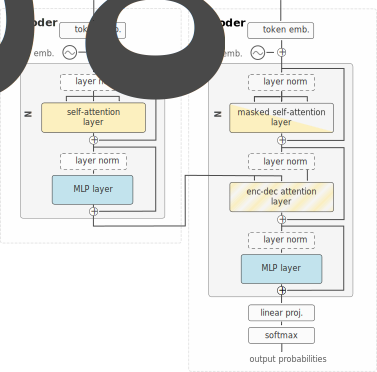
\includegraphics[width=0.9\textwidth]{img/transformer.pdf}
    \caption{An encoder-decoder variant of the Transformer architecture. Adapted from \href{https://github.com/bbycroft/llm-viz/blob/main/src/llm/intro-image.svg}{https://github.com/bbycroft/llm-viz}.}
    \label{fig:transformer}
\end{figure*}


As shown in \autoref{fig:transformer}, the original Transformer architecture follows the encoder-decoder framework. The encoder consists of $N_e$ layers, the decoder of $N_d$ layers. The decoder layers have the following differences:
\begin{itemize}
    \item Each layer contains another sublayer called the \emph{encoder-decoder attention}. In contrast to the self-attention mechanism, the \emph{keys} and \emph{values} come from the last layer of the encoder, enabling the decoder to attend to the encoded sequence (analogically to the original attention mechanism).
    \item The self-attention is \emph{masked} so that each token can collect information only from the preceding tokens. This is to preserve the temporal casuality during left-to-right text generation, in which the following tokens are not yet decoded.
\end{itemize}
After the last decoder layer, the hidden states are projected into a matrix of size $\mathbb{R}^{|V|\times n}$ and normalized using softmax, producing a probability distribution over the vocabulary for each input token.

In each step, we train the model maximize the log probability (i.e., minimize the negative log probability) of the ground truth token $y_i$ given the previous sequence of tokens:
\begin{align}
    \operatorname{loss}_i = -\log P_\theta(y_i|y_1, \hdots, y_{i-1})
\end{align}

\paragraph{Text Generation} The prevalent approach for text generation with transformer models is using \textit{autoregressive left-to-right decoding}. The decoding process starts by feeding a special \texttt{<s>} token into the decoder and then iteratively selecting the \emph{i}-th token based on the probability distribution for the \emph{i}-th position. The procedure is outlined in Algorithm \ref{alg:decoding}.
\begin{algorithm}[ht]
    \begin{algorithmic}[1]
        \State Initialize:
        \Statex{  $Y= \texttt{<s>}, y_t = \texttt{<s>}$ \Comment{Output sequence, current token}}
        \While{$y_t \neq \texttt{</s>}$}
        \State Predict next token probability distribution: $p(y_t | Y)$
        \State Sample next token: $t \sim p(y_t | Y)$
        \State Update output sequence: $Y = Y \cup y_t'$
        \EndWhile
        \State Return $Y$
    \end{algorithmic}
    \caption{Autoregressive decoding}
    \label{alg:decoding}
\end{algorithm}

\noindent The step of sampling the next token can be realized in multiple ways:
\begin{itemize}
    \item \textbf{Greedy decoding}: Select the most probable token.
    \item \textbf{Beam search}: Extend the $k$ most probable sequences from the previous step with the next tokens, keep the $k$ most probable sequences for the next step.
    \item \textbf{Top-$k$ sampling}: Sample the next token from the $k$ most probable tokens.
    \item \textbf{Top-$p$ sampling} \cite{holtzman2019curious}: Sample the next token from the tokens with cumulative probability $p$.
\end{itemize}
While the greedy decoding and beam search are used to decode more probable sentences, the sampling algorithms are used for decoding more creative outputs.

\subsection{Pretrained Language Models}
\label{sec:plms}
Having a generic way to learn patterns from data is only a part of the equation: we also need the data itself. The
\paragraph{Encoder Models}

\paragraph{Encoder-Decoder Models}

\paragraph{Decoder Models}

\subsection{Large Language Models}
\label{sec:llms}
\section{Data-to-Text Generation}
\label{sec:d2t}
\subsection{Rule-based Approaches}
\label{sec:rule-d2t}
\subsection{Neural Approaches}
\label{sec:neural-d2t}
\subsection{Datasets}
\label{sec:datasets}
\subsection{Evaluation Metrics}
\label{sec:evaluation}
\chapter{Low-Resource Data-to-Text Generation}
\label{chap:low-res}


In this chapter, we introduce three approaches for low-resource \ac{d2t} generation based on \acp{plm}. By \emph{low-resource}, we mean using as little data as possible for generating fluent and accurate text. We develop approaches that leverage the general-domain pretraining of \acp{plm} in order to generate texts in domains with thousands, hundreds, or even zero training examples.

The data we focus on are \acs{rdf} (\Acl{rdf}) triples from factual knowledge graphs and meaning representations in dialogue systems. The main feature of these kinds of data is that we always want to verbalize the whole input. For larger data, we would need a separate content selection component, but our approaches are generalizable to other kinds of data which fulfill this requirement.

The simplest setting, presented in \autoref{sec:finetuning}, consists of finetuning a pretrained transformer encoder-decoder model. For finetuning the model, we need approximately thousands of in-domain examples. We show that this baseline is powerful, achieving competitive results on a shared task for generating knowledge graph descriptions. On top of that, we show that this approach generalizes to other languages than English, namely Russian.

In \Cref{sec:iterative,sec:pipeline}, we then present approaches which can generate texts with even \emph{more limited amount} of in-domain training examples. Our key idea is to use a \ac{plm} only as a tool for improving text fluency \emph{regardless of the content}, and delegating (possibly crude and basic, but factually correct) verbalization of the content to other, simpler tools. \autoref{sec:iterative} shows an approach using a text-editing model trained on iteratively fusing simple templates, which has a limited vocabulary focused on sentence fusion. The limited vocabulary and training objective pushes the model towards generating factually correct sentences. In \autoref{sec:pipeline}, we also add an ordering and aggregation step for generating more fluent texts. For each of these steps, we can train a \ac{plm} entirely on general-domain operations, reducing the need for in-domain examples to zero.

% \section{Motivation}
% \label{sec:low-res-mot}
\section{Finetuning PLMs}
\label{sec:finetuning}

\begin{refbox}
    This section is based on the paper \emph{Train Hard, Finetune Easy: Multilingual Denoising for RDF-to-Text Generation} \cite{kasnerTrainHardFinetune2020}, joint work with Ondřej Dušek, published in the Proceedings of the 3rd International Workshop on Natural Language Generation from the Semantic Web (WebNLG+) at INLG 2020.
\end{refbox}


We introduce a simple approach for generating knowledge graph descriptions. Our approach is based on finetuning a multi-lingual \ac{plm} on linearized graphs and the accompanying human-written descriptions from the WebNLG dataset. In the WebNLG+ Shared Task, our model placed in the first third of the leaderboard for English and first or second for Russian on automatic metrics, and in the best or second-best system cluster on human evaluation.

\subsection{WebNLG+ Shared Task}
\label{sec:webnlgp}
The WebNLG Challenge 2020\footnote{\url{https://synalp.gitlabpages.inria.fr/webnlg-challenge/challenge_2020/}} (WebNLG+; \citealp{ferreira20202020}) was the second edition of the shared task in graph-to-text generation. The task was based on the WebNLG dataset, which contains subgraphs from the DBpedia knowledge graph. Each subgraph is described by a set of \ac{rdf} triples and accompanied with crowdsourced text descriptions (see \autoref{sec:datasets}). On top of the original challenge \cite{gardentWebNLGChallengeGenerating2017}, WebNLG+ included a separate track of generating texts in Russian, in which we also participated.


\subsection{Problem Formulation}
\label{sec:mbart}
Our input is a set of \ac{rdf} triples $x \in X$, where each triple $x = (s, p, o)$ describes the relation $p$ between the entities $s$ and $o$ in the knowledge graph. Our target output $Y$ is a fluent and semantically accurate natural language description of $X$.


We formulate the task as \emph{sequence-to-sequence} generation. First, we linearize the input sequence in the default order. We select two arbitrary separator tokens: one to delimit the contituents of the triple and another to delimit individual triples. Using the linearized sequence as an input and the target text, we finetune a pretrained encoder-decoder model using the cross-entropy objective (see \autoref{sec:transformer}). We use the finetuned model to generate the target texts using autoregressive decoding (see Algorithm~\ref{alg:decoding}).

% 


\subsection{Implementation}
\paragraph{Data Preprocessing} We use the provided XML WebNLG data reader\footnote{\url{https://gitlab.com/webnlg/corpus-reader}} to load and linearize the triples. For each triple, we use the \texttt{flat\_triple()} method which converts each triple into the ``\texttt{s $\vert$ p $\vert$ o}'' string, using a pipe (``$\vert$'') as a separator. We use another token not present in the training data (``$\blacktriangleright$'') for delimiting individual triples to avoid extending the model vocabulary.\footnote{Our choice of the separators is arbitrary, as we will adapt the model to account for our separators.
    % Works such as \TODO{cite} or \TODO{cite} show that the choice of separators is not important.
} We linearize the triples in their default order. For the input to the model, we tokenize the data using SentencePiece tokenizer \citep{kudo2018sentencepiece} trained on the training dataset, using a vocabulary of 250,000 subword tokens.

\paragraph{Model}
We use mBART \cite{liuMultilingualDenoisingPretraining2020}, a multilingual \ac{plm} based on BART, a transformer model pretrained on text denoising (see \autoref{sec:plms}).
% In pretraining, the noise function of mBART replaces text spans of arbitrary length with a mask token (35\% of the words in each instance) and permutes the order of sentences. 
The model uses 12 layers for the encoder and 12 layers for the decoder ($\sim$680M parameters), and it is pretrained on the large-scale CC25 corpus extracted from Common Crawl, which contains data in 25 languages \citep{wenzek2020ccnet}.



\paragraph{Training} We finetune the pre-trained \texttt{mbart.CC25} model from the \textsc{fairseq} toolkit \citep{ott2019fairseq} using the default parameters.\footnote{We use dropout 0.3, attention dropout 0.1, and 1024 tokens per batch. We set the initial learning rate to 0.0003 and use polynomial decay with 2500 warmup steps. We train the model using the Adam optimizer \cite{kingma2014adam} with $\beta_1=0.9, \beta_2=0.98$ and $\varepsilon=1e-06$. For the full setup, see \url{https://github.com/facebookresearch/fairseq/tree/main/examples/mbart}.} We change the total number of updates from 40k to 10k to reflect the smaller size of our data. We train a separate version of mBART for each language: $\text{mBART}_{\text{en}}$ on English inputs and English outputs, and $\text{mBART}_{\text{ru}}$ on English inputs and Russian outputs.



\subsection{Results}

\begin{table*}[t]
    \footnotesize
    \centering
    \begin{tabular}{@{}lp{12.7cm}@{}}
        \textbf{input}    & \texttt{Piotr\_Hallmann | weight | 70.308 }  $\blacktriangleright$ \texttt{ Piotr\_Hallmann | birthDate | 1987-08-25} \\
        \textbf{out (en)} & Born on August 25th 1987, Piotr Hallmann has a weight of 70.308.                                                      \\
        \midrule
        \textbf{in}       & \texttt{Ciudad\_Ayala | populationMetro | 1777539}                                                                    \\
        \textbf{out (en)} & The population metro of Ciudad Ayala is 1777539.                                                                      \\
        \midrule
        \textbf{in}       & \texttt{Bakewell\_tart | ingredient | Frangipane}                                                                     \\
        \textbf{out (ru)} & Франжипан - один из ингредиентов тарта Бейквелл.                                                                      \\[0.1cm]
        \textbf{transcr.} & Franzhipan - odin iz ingredientov tarta Bejkvell.                                                                     \\
        \textbf{transl.}  & Frangipane is one of the ingredients of the Bakewell tart.                                                            \\
    \end{tabular}
    \caption{Example outputs from the mBART model(s) finetuned for \ac{rdf}-to-text generation. (1) The model can work with unseen entities, dates and numbers. (2) The model is quite robust to unseen properties, such as \texttt{populationMetro}. However, the surface form of the property deviates too much from its meaning and the sentence is incorrect. (3) The model trained on Russian targets can use English data to form sentences in Russian, transcribing the entities to Cyrillic.}
    \label{tab:mbart:examples}
\end{table*}

We report on WebNLG automatic and human evaluation results, as well as our own error analysis.

\paragraph{Automatic Metrics}
The results of our approach for English are shown in \autoref{tab:mbart:results-en}, comparing to the baseline.
% \footnote{See \url{https://gerbil-nlg.dice-research.org/gerbil/webnlg2020results} for full results.} 
We can see that our approach beats the baseline in all metrics and places in the first third of the submissions. While it does lose performance on unseen categories, the drop is not as dramatic as for many other competing approaches.

The results for Russian are shown in \autoref{tab:mbart:results-ru}. There were fewer submissions for Russian, and our system not only beats the baseline by a large margin (as did all competing submissions), but it is able to rank first in 2 metrics out of 4 (BLEU, BERTScore) and second in the remaining ones.

\paragraph{Human Evaluation}

The challenge organizers ran a human evaluation campain, where annotators were asked to rate the texts for data coverage, relevance, correctness, text structure and fluency.  Each criterion has been rated with a number in the range from 0 (completely disagree) to 100 (completely agree). The scores were clustered into groups (1-5; 1 being the best) among which there are no statistically significant differences according to the Wilcoxon rank-sum test \citep{wilcoxon1992individual}.

Our systems placed in the top clusters (1 or 2) for both English and Russian. For English, our $\text{mBART}_{\text{en}}$ system ranks first for all the categories in \textit{seen domains}, and first or second in \textit{unseen entities} and \textit{unseen domains}. In total, our English system achieved rank 1 for relevance, correctness and text structure, and rank 2 for data coverage and fluency. For Russian, our $\text{mBART}_{\text{ru}}$ system ranks second for correctness and first in all other categories.


\begin{table*}[t]
    \footnotesize\centering
    \begin{tabular}{llcccccccccc}\toprule
                                     &          & \multicolumn{2}{c}{\bf BLEU} & \multicolumn{2}{c}{\bf METEOR} & \multicolumn{2}{c}{\bf ChrF++} & \multicolumn{2}{c}{\bf BERTScore} & \multicolumn{2}{c}{\bf BLEURT}                                     \\\midrule
        \multirow{2}{*}{All}         & Ours     & 50.34                        & (10)                           & 0.398                          & (8)                               & 0.666                          & (8)  & 0.951 & (8)  & 0.57 & (8)  \\
                                     & Baseline & 40.57                        & (14)                           & 0.373                          & (15)                              & 0.621                          & (15) & 0.943 & (14) & 0.47 & (12) \\\midrule
        \multirow{2}{*}{Seen Cat.}   & Ours     & 59.13                        & (10)                           & 0.422                          & (10)                              & 0.712                          & (9)  & 0.960 & (9)  & 0.58 & (14) \\
                                     & Baseline & 42.95                        & (31)                           & 0.387                          & (27)                              & 0.650                          & (28) & 0.943 & (31) & 0.41 & (31) \\\midrule
        \multirow{2}{*}{Unseen Cat.} & Ours     & 42.24                        & (10)                           & 0.375                          & (13)                              & 0.617                          & (10) & 0.943 & (11) & 0.52 & (10) \\
                                     & Baseline & 37.56                        & (12)                           & 0.357                          & (15)                              & 0.584                          & (15) & 0.940 & (12) & 0.44 & (12) \\\midrule
        \multirow{2}{*}{Unseen Ent.} & Ours     & 51.23                        & (4)                            & 0.406                          & (8)                               & 0.687                          & (7)  & 0.959 & (8)  & 0.63 & (8)  \\
                                     & Baseline & 40.22                        & (17)                           & 0.384                          & (15)                              & 0.648                          & (15) & 0.949 & (13) & 0.55 & (12) \\\bottomrule
    \end{tabular}
    \caption{Results of $\text{mBART}_{\text{en}}$ (all data, seen categories, unseen categories, unseen entities), compared to the baseline. The numbers in brackets show the rank of each model (out of 35 submissions) with respect to the given metric.}
    \label{tab:mbart:results-en}
\end{table*}
\begin{table*}[t]
    \footnotesize\centering
    \begin{tabular}{llcccccccc}\toprule
                 & \multicolumn{2}{c}{\bf BLEU} & \multicolumn{2}{c}{\bf METEOR} & \multicolumn{2}{c}{\bf ChrF++} & \multicolumn{2}{c}{\bf BERTScore}                               \\\midrule
        Ours     & 52.93                        & (1)                            & 0.672                          & (2)                               & 0.677 & (2)  & 0.909 & (1)  \\
        Baseline & 23.53                        & (12)                           & 0.461                          & (12)                              & 0.511 & (12) & 0.836 & (12) \\\bottomrule
    \end{tabular}
    \caption{Results of $\text{mBART}_{\text{ru}}$, compared to the baseline. The numbers in brackets show the rank of each model (out of 12 submissions) if ordered by the given metric.}
    \label{tab:mbart:results-ru}
\end{table*}

\paragraph{Manual Analysis}
To better understand the nature of errors made by our system, we manually inspected a sample of 50 outputs in each language.\footnote{Automatic back-translation to English was used to facilitate understanding of Russian.} We found factual errors in 12 English outputs, mostly concentrated along the unseen categories (\emph{Scientist}, \emph{Movie}, \emph{Musical Record}). The model tends to describe musical works and movies in terms of written works (“written”, “published” etc.), i.e., the closest seen category. There are also several swaps in roles of the entities (e.g., “is to southeast” instead of “has to its southeast”, “follows” instead of “is followed by” etc.).

In a few cases, the model hallucinates a relation not specified in the data (e.g., “born on January 1, 1934 in Istanbul” when a date of birth and current residence is given, not the birthplace) or is not able to infer background knowledge not given on the input (it talks about a dead person in the present tense).
% The swaps in roles and hallucinated relations also occured in Russian; in addition, we found a hallucinated (correct) airport name and a few forgotten ingredients for a dish from a long list. 
Factual errors in Russian were less frequent (9 sentences), which is expected as there are no unseen categories. Moreover, the system shows an impressive performance at translating entity names from the English \ac{rdf} into Russian.

We further found 10 outputs with suboptimal phrasing in English and 9 in Russian, where the model did not connect properties of the same type in a coordination (e.g., two musical genres for a record) or gave numbers without proper  units (e.g., “runtime of 89.0” or “area of 250493000000.0”).

\paragraph{Discussion}
Our solution benefits from the pretrained representations of the mBART model. Multilingual pretraining allows us to use a single architecture for both English and Russian. However, English and Russian are the two most represented languages in the mBART pre-training corpora (ca. 300 GB of data each) and the performance of our model would probably be lower with low-resource languages.

The performance of our model is also noticeably lower on categories unseen in training, and it is prone to swapping relations of entities or hallucinating relations. Even though the longest examples in the WebNLG dataset fit into the model, the length of the input sequence is still limited and the model does not generalize for inputs of arbitrary size.





\section{Iterative Sentence Fusion}
\label{sec:iterative}

\begin{refbox}
    This section is based on the paper \emph{Data-to-Text Generation with Iterative Text Editing} \cite{kasnerDatatoTextGenerationIterative2020}, joint work with Ondřej Dušek, published in the Proceedings of the 13th International Conference on Natural Language Generation (INLG 2020).
\end{refbox}

We present an approach for generating semantically accurate texts from structured data in low-resource settings. Our approach builds on a text-editing model trained on the task of \emph{sentence fusion}. We first transform individual data items to text using trivial templates, and iteratively improve the resulting text using the sentence fusion model, filtering, and re-ranking.  Our approach gets lower scores on lexical similarity metrics on WebNLG and E2E datasets than the state-of-the-art approaches; however, it achieves high levels of semantic accuracy due to the limited scope of the sentence fusion model and guaranteed presence of the entities. We also demonstrate that our task formulation opens up the possibility for zero-shot \ac{d2t} generation by training a model on a general-domain dataset for sentence fusion. The code for the experiments is available on Github.\footnote{\url{https://github.com/kasnerz/d2t_iterative_editing}}


\subsection{Motivation}
\label{sec:text-editing}
Our goal is to improve the semantic accuracy \ac{d2t} generation. Other works have pursued this goal, e.g., by adapting the decoding algorithm \cite{tianStickingFactsConfident2020}, improving robustness of the model by injecting noise in its hidden states \cite{kedzie_good_2019}, or self-training with a natural language understanding model \cite{nieSimpleRecipeReducing2019}. Our approach is inspired by the systems which use a \emph{generate-then-rerank} approach \citep{dusekSequencetoSequenceGenerationSpoken2016,juraska_deep_2018}, e.g. using a classifier \cite{harkousHaveYourText2020}, to filter incorrect outputs.

To generate outputs with sufficient semantic accuracy for the filtering step, we take advantage of three facts: (1) we can lexicalize individual data items using trivial templates, (2) concatenating the lexicalizations tends to produce an unnatural sounding but semantically accurate output, and (3) a \ac{plm} trained on improving the output fluency can be used for combining the lexicalizations.

% \textsc{LaserTagger} \cite{malmi2019lasertagger}, which we use in our approach, is a sequence tagging model based on the transformer architecture with BERT \cite{devlinBERTPretrainingDeep2019} as the encoder backbone. Other recent text-editing models without a pre-trained backbone include EditNTS \citep{dong} and Levenshtein Transformer \citep{gu2019levenshtein}.

% Concurrently with our work, \citet{kale2020few} explored using templates for dialogue response generation. %\ODdel{Unlike our work,} 
% They use the sequence-to-sequence T5 model \citep{raffel2019exploring} to generate the output text from scratch instead of iteratively editing the intermediate outputs, which leaves less control over the model.


\subsection{Our Approach}
\label{sec:text-editing-exp}
We focus on data structured as \ac{rdf} triples.\footnote{Later, we also trivially extend our approach to key-value pairs.} In our approach, we start from single-triple templates and iteratively fuse them into the resulting text while filtering and reranking the results. We first detail the main components of our system (template extraction, sentence fusion, \ac{plm} scoring) and then give the overall description of the generation algorithm.

\begin{figure*}[t]
    \centering
    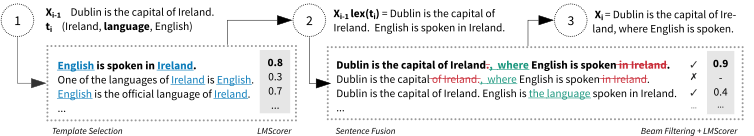
\includegraphics[width=\textwidth]{img/d2t_text_editing}
    \caption{A single iteration of our algorithm for iterative \ac{d2t} generation. In Step 1, the template for the triple is selected and filled. In Step 2, the sentence is fused with the template. In Step 3, the result for the next iteration is selected from the beam by filtering and language model scoring.}\label{fig:iterative:alg}
\end{figure*}



\paragraph{Template Extraction}
We collect a set of templates for each unique predicate. We use two approaches: (a) handcrafting the template manually for each predicate in the training set, and (b) automatically extracting the template from the lexicalizations of the examples  in the training set. For unseen predicates, we add a single fallback template: \textit{The <predicate> of <subject> is <object>.}


\paragraph{Sentence Fusion}
We train a model for the task of \emph{sentence fusion}, i.e., combining sentences into a coherent text \cite{barzilay2005sentence}.
%We train an independent in-domain sentence fusion model for each dataset. 
To construct the training data for the model, we select pairs of examples $(X, X')$ and their corresponding text descriptions $(Y, Y')$ from the original training set such that the examples consist of $(k, k+1)$ triples and have $k$ triples in common. This leaves us with an extra triple $x_{k+1}$ present only in $X'$. For each training example, we use the concatenated sequence $Y \mathrm{lex}(x_{k+1})$ as a source and the sequence $Y'$ as a target, where $\mathrm{lex}(x_{k+1})$ denotes lexicalizing the triple $x_{k+1}$ using an appropriate template.
As a result, the model learns to integrate $Y$ and $x_{k+1}$ into a single coherent expression.


\paragraph{PLM Scoring} For re-ranking the text, we use an additional component for computing text fluency, which we refer to as \textsc{LMScorer}.
As described in \autoref{sec:evaluation}, we use perplexity of the text under a a \ac{plm}, computing the score of the output text $Y$ composed of tokens $(y_1, \ldots, y_n)$ as a geometric mean of the token conditional probability:
\begin{align}
    \operatorname{score}(Y) = \Bigg( \prod_{i=1}^{n}{P(y_i|y_1, \ldots, y_{i-1})} \Bigg)^{\frac{1}{n}}.
\end{align}




\paragraph{Generation Algorithm}
The input of the algorithm (\autoref{fig:iterative:alg}) is a set of $T$ ordered triples. First, we lexicalize the triple $x_0$ to get the output text $Y_0$ by filling the available templates and using the template with the best score from \textsc{LMScorer}.
% This promotes templates which sound more natural for particular values.
In each of the following steps $i=(1, \ldots, T-1)$, we lexicalize the triple $x_i$ and concatenate it with $Y_{i-1}$.  For improving the fluency of the text, we use the sentence fusion model with beam search to produce $k$ hypotheses. We filter and re-rank the hypotheses, getting $Y_{i}$ (see the next paragraph), and proceed to the next step. The output of the algorithm is the text $Y_{T-1}$ from the final step.


\paragraph{Filtering and Re-ranking} In each decoding step, we remove hypotheses in the beam missing any entity from the input data using a simple heuristic based on string matching. Next, we rescore the remaining hypotheses in the beam with \textsc{LMScorer} and set the hypothesis with the best score as $Y_{i}$. In case there are no sentences left in the beam after the filtering step, we let $Y_{i}$ be the text in which the lexicalized $x_i$ is appended after $Y_{i-1}$ without sentence fusion, ensuring the semantic accuracy of the text.

%For the E2E dataset, we first try to find a pair of predicates for which there is a template extracted from the data, and only use the handcrafted templates for the single predicates in the subsequent steps. 
%The final beam filtering step is a simple heuristic, checking if all entities from the input triples are present in the output.


\subsection{Implementation}


\begin{table}[t]
    \centering\footnotesize
    \begin{tabular}{lllll}
        \textbf{dataset} & \textbf{method} & \textbf{predicate}          & \textbf{example \#1}                            & \textbf{example \#2}                     \\\midrule
        WebNLG           & extracted       & \texttt{foundedBy}          & \textit{$o$ was the founder of $s$.}            & \textit{$s$ was founded by $o$.}         \\
        E2E              & extracted       & \texttt{area}+\texttt{food} & \textit{$s$ offers $o_2$ cuisine in the $o_1$.} & \textit{$s$ in $o_1$ serves $o_2$ food.} \\
        E2E              & manual          & \texttt{near}               & \textit{$s$ is located near $o$.}               & \textit{$o$ is close to $s$.}
    \end{tabular}
    \caption{Examples of templates we used in our experiments. The templates for the single predicates in the WebNLG dataset and the pairs of predicates in the E2E dataset are extracted automatically from the training data; the templates for the single predicates in E2E are created manually.}
    \label{tab:iterative:templates_ex}
\end{table}


\paragraph{Template Extraction} We experiment with the WebNLG and E2E datasets (see \autoref{sec:datasets}). For WebNLG, we extract the templates from the training examples containing only a \textit{single} triple. In the E2E dataset, there are no such examples; therefore we first extract the templates for \textit{pairs} of predicates, using them as a starting point for the algorithm in order to leverage the lexical variability in the data (manually filtering out the templates with semantic noise), and we also create a small set of templates for each \textit{single} predicate manually, using them in the subsequent steps of the algorithm.\footnote{In the E2E dataset, the data is in the form of key-value pairs. We transform the data to \ac{rdf} triples by using the name of the restaurant as a \textit{subject} and the rest of the pairs as \textit{predicate} and \textit{object}. This creates \textit{n-1} triples for \textit{n} pairs.} See \autoref{tab:iterative:templates_ex} for examples of templates we used in our experiments.

\paragraph{Sentence Fusion Model} We base our sentence fusion model on the text-editing model \textsc{LaserTagger} \cite{malmi2019lasertagger}. \textsc{LaserTagger} generates outputs by tagging inputs with edit operations (\texttt{KEEP} a token, \texttt{DELETE} a token, and \texttt{ADD} a phrase before the token), which makes it suitable for tasks where the output highly overlaps with the input. An important feature of \textsc{LaserTagger} is the limited size of its vocabulary, which consists of $l$ most frequent (possibly multi-token) phrases used to transform inputs to outputs in the training data. After the vocabulary is precomputed, all infeasible examples in the training data are filtered out. At the cost of limiting the number of training examples, this filtering makes the training data cleaner by removing outliers. The limited vocabulary also makes the model less prone to hallucinations errors.

\paragraph{LMScorer} As the \textsc{LMScorer} backend, we use the pre-trained GPT-2 language model \citep{radford2019language} from the Transformers repository\footnote{\url{https://github.com/huggingface/transformers}} \citep{wolf2019HuggingFacesTS}. We compute the perplexity scores using the \textit{lm-scorer}\footnote{\url{https://github.com/simonepri/lm-scorer}} package.





\begin{table*}[t]% \begin{adjustbox}{max width=\textwidth}
    \centering\footnotesize
    \begin{tabular}{lcccc<{\hspace{2mm}}c>{\hspace{2mm}}cccc} \toprule
                         & \multicolumn{4}{c}{\bf WebNLG} &            & \multicolumn{4}{c}{\bf E2E}                                                                                                                                                                          \\
        \cmidrule{2-5} \cmidrule{7-10}
                         & {\it BLEU}                     & {\it NIST} & \hspace{-1mm}{\it METEOR}\hspace{-1mm} & \hspace{-1mm}{\it ROUGE$_L$}\hspace{-1mm} &  & {\it BLEU} & {\it NIST} & \hspace{-1mm}{\it METEOR}\hspace{-1mm} & \hspace{-1mm}{\it ROUGE$_L$}\hspace{-1mm} \\
        {\bf baseline}   & 0.277                          & 6.328      & 0.379                                  & 0.524                                     &  & 0.207      & 3.679      & 0.334                                  & 0.401                                     \\
        {\bf zero-shot } & 0.288                          & 6.677      & 0.385                                  & 0.530                                     &  & 0.220      & 3.941      & 0.340                                  & 0.408                                     \\
        {\bf w/fusion }  & 0.353                          & 7.923      & 0.386                                  & 0.555                                     &  & 0.252      & 4.460      & 0.338                                  & 0.436                                     \\
        {\bf SFC }       & 0.524                          & -          & 0.424                                  & 0.660                                     &  & 0.436      & -          & 0.390                                  & 0.575                                     \\
        {\bf T5 }        & 0.571                          & -          & 0.440                                  & -                                         &  & -          & -          & -                                      & -                                         \\ \bottomrule
    \end{tabular}
    \caption{Results of automatic metrics on the WebNLG and E2E test sets. The comparison is made with the results from the papers on the Semantic Fidelity Classifier (SFC; \citealp{harkousHaveYourText2020}) and the finetuned T5 model (T5; \citealp{kaleTexttoTextPreTrainingDatatoText2020}), state-of-the-art approaches at that time.}
    \label{tab:results}
    % \end{adjustbox}
\end{table*}



\subsection{Experiments}
\paragraph{Base Experiments} As a \emph{baseline}, we generate the best templates according to \textsc{LMScorer} without applying the sentence fusion (i.e., always using the fallback). For the \emph{sentence fusion} experiments, we use \textsc{LaserTagger} with the autoregressive decoder with a beam of size 10. We use all reference lexicalizations and the vocabulary size $V=100$, following our preliminary experiments. We finetune the model for 10,000 updates with batch size 32 and learning rate $2 \times 10^{-5}$.
For the beam filtering heuristic, we check for the presence of entities by simple string matching in WebNLG; for the E2E dataset, we use a set of regular expressions from \citet{dusekSemanticNoiseMatters2019}. We process the triples in their default order.

\paragraph{Zero-shot Experiment} Additionally, we conduct a \textit{zero-shot} experiment. We train the sentence fusion model with the same setup, but instead of the in-domain datasets, we use a subset of the balanced-Wikipedia portion of the \textsc{DiscoFuse} dataset \cite{geva-etal-2019-discofuse}. In particular, we use the discourse types which frequently occur in our datasets, filtering the discourse types which are not relevant for our use-case.


% \vspace{-3mm}
\subsection{Results}

\begin{table*}[t] \footnotesize
    \begin{tabular}{l p{12cm}}
        \textbf{Triples}   & \textit{(Albert Jennings Fountain, deathPlace, New Mexico Territory); (Albert Jennings Fountain, birthPlace, New York City); (Albert Jennings Fountain, birthPlace, Staten Island)} \\ \midrule
        \textbf{Step \#0}  & Albert Jennings Fountain died in New Mexico Territory.                                                                                                                              \\
        \textbf{Step \#1}  & Albert Jennings Fountain, who died in New Mexico Territory, was born in \greenund{New York City}.                                                                                   \\
        \textbf{Step \#2}  & Albert Jennings Fountain, who died in New Mexico Territory, was born in New York City, \greenund{Staten Island}.                                                                    \\ \midrule
        \textbf{Reference} & Albert Jennings Fountain was born in Staten Island, New York City and died in the New Mexico Territory.
    \end{tabular}
    \caption{An example of correct behavior of the algorithm on the WebNLG dataset. Newly added entities are underlined, the output from Step \#2 is the output text.}\label{tab:iterative:output}
\end{table*}


\paragraph{Accuracy vs.\ Fluency}
The scores from the automatic metrics lag behind the state-of-the-art, although both the fusion and the zero-shot approaches show improvements over the baseline. Our approach ensures zero entity errors, since the entities are filled verbatim into the templates and in case an entity is missing in the whole beam, a fallback is used instead. Semantic inconsistencies still occur, e.g.\ if a verb or function words are missing.

The fused sentences in the E2E dataset, where all the objects are related to a single subject, often lean towards compact forms, e.g.: \textit{Aromi is a family friendly chinese coffee shop with a low customer rating in riverside}. On the contrary, the sentence structure in WebNLG mostly follows the structure from the templates and the model performs minimal changes to fuse the sentences together. See \autoref{tab:iterative:output} for examples of the system outputs. Out of all steps, 28\% are fallbacks (no fusion is performed) in WebNLG and 54\% in the E2E dataset. % v anglictine se za '\%' nedela mezera
The higher number of fallbacks in the E2E dataset can be explained by a higher lexical variability of the references, together with a higher number of data items per example in the E2E dataset, making it harder for the model to maintain the text coherency over multiple steps.

\paragraph{Templates} On average, there are 12.4 templates per predicate in WebNLG and 8.3 in the E2E dataset. In cases where the set of templates is more diverse, e.g.\ if the template for the predicate \textit{country} has to be selected from \{\textit{<subject> is situated within <object>, <subject> is a dish found in <object>}\}, \textsc{LMScorer} helps to select the semantically accurate template for the specific entities. The literal copying of entities can be too rigid in some cases, e.g.\ \textit{Atatürk Monument (İzmir) is made of ``Bronze''}, but these disfluencies can be improved in the fusion step.

\paragraph{Reordering} \textsc{LaserTagger} does not allow arbitrary reordering of words in the sentence, which can limit the expressiveness of the sentence fusion model. Consider the example in \autoref{fig:iterative:alg}: in order to create a sentence \textit{English is spoken in Dublin, the capital of Ireland}, the model has to delete and re-insert at least one of the entities, e.g.\ \textit{English}, which has to be present in the vocabulary.

\paragraph{Domain Independence} The zero-shot model trained on \textsc{DiscoFuse} is able to correctly pronominalize or delete repeated entities and join the sentences with conjunctives, e.g.\ \textit{William Anders was born in British Hong Kong\underline{, and was} a member of the crew of Apollo 8}. While the model makes only a limited use of sentence fusion, it makes the output more fluent while keeping strong guarantees of the output accuracy.

\subsection{Discussion}
% Building a high-quality sentence fusion model, which lies at the core of our approach, remains a challenge \cite{lebanoff2020learning}. Our simple extractive approach relying on existing D2T datasets may not produce sufficient amount of clean data. On the other hand, the phenomena covered in the \textsc{DiscoFuse} dataset are too narrow for the fully general sentence fusion. We believe that training the sentence fusion model on a larger and more diverse sentence fusion dataset, built e.g. in an unsupervised fashion \cite{lebanoff-etal-2019-scoring}, is a way to improve the robustness of our approach.

% Fluency of the output sentences may be also improved by allowing more flexibility for the order of entities, either by including an ordering step in the pipeline \citep{moryossef2019astep}, or by using a text-editing model that is capable of explicit reordering of words in the sentence \cite{mallinson2020felix}. Splitting the data into smaller batches (i.e. setting an upper bound for the number of sentences fused together) could also help to improve the consistency of results with a higher number of data items.

% Our string matching heuristic is quite crude and may lead to a high number of fallbacks. Introducing a more precise heuristic, such as a semantic fidelity classifier \citep{harkous2020have}, or a model trained for natural language inference \citep{dusek2020nli} could help to promote lexical variability of the text.

% Finally, we note that the text-editing paradigm allows to visualize the changes made by the model, introducing the option to accept or reject the changes at each step, and even build a set of custom rules on top of the individual edit operations based on the affected tokens. This flexibility could be useful for tweaking the model manually for a production system.


% \subsection{Conclusions}
% We proposed a simple and intuitive approach for D2T generation, splitting the process into two steps: lexicalization of data and improving the text fluency. A trivial lexicalization helps to promote fidelity and domain independence while delegating the subtle work with language to neural models allows to benefit from the power of general-domain pre-training. While a straightforward application of this approach on the WebNLG and E2E datasets does not produce state-of-the-art results in terms of automatic metrics, the results still show considerable improvements above the baseline. We provided insights into the behavior of the model, highlighted its potential benefits, and proposed the directions for further improvements.


\section{Pipeline of Text-to-Text Neural Modules}
\label{sec:pipeline}
\begin{refbox}
    This section is based on the paper \emph{Neural Pipeline for Zero-Shot Data-to-Text Generation} \cite{kasner2022neural}, joint work with Ondřej Dušek, published in the Proceedings of the 60th Annual Meeting of the Association for Computational Linguistics (ACL 2022).
\end{refbox}

In this section, we further develop the approach from \autoref{sec:iterative} for generating semantically accurate text from structured data. The main limitation of the previous approach, which was based on iterative transformations of simple templates, was the limited fluency of the output texts. To improve text fluency, we propose adding ordering and aggregation, making the process a three-step pipeline. We also propose a way to make each of these steps trainable on a generic synthetic corpus. We confirm that on WebNLG and E2E dataset, our approach can get lower rates of omissions and hallucinations than prior approaches according to a semantic accuracy metric (on the E2E dataset, the rate is close to zero), while achieving levels of lexical similarity comparable to some of the prior systems; all of this without the need for in-domain training data. Our code and data is available on Github.\footnote{\url{https://github.com/kasnerz/zeroshot-d2t-pipeline}}

% an approach for transforming the templates based on a sequence of modules trained on general-domain text-based operations: ordering, aggregation, and paragraph compression. We train \acp{plm} for performing these operations on a synthetic corpus \textsc{WikiFluent} which we build from English Wikipedia. Our experiments on WebNLG and E2E show that our approach enables \ac{d2t} generation from \ac{rdf} triples in zero-shot settings. Our code and data is available on Github.\footnote{\url{https://github.com/kasnerz/zeroshot-d2t-pipeline}}

\subsection{Motivation}
Our experiments in \autoref{sec:iterative} with iterative sentence fusion led to several observations:

\begin{enumerate}
    \item The fixed order of triples limits the expressivity of the model, leading to unnatural outputs.
    \item Using the sentence fusion model on every sentence boundary tends to produce sentences which are too compact.
    \item Instead of specialized architectures such as text-editing models, state-of-the-art approaches for text generation are based on autoregressive models \cite{kaleTexttoTextPreTrainingDatatoText2020,ribeiroInvestigatingPretrainedLanguage2020}.
\end{enumerate}

Following these observations, we improve our approach by (1) inserting a triple-ordering step in the process, (2) replacing the sentence fusion by paragraph compression, and (3) basing the approach on trainable autoregressive models.


Our approach follows the idea of pipeline-based approaches (see \autoref{sec:d2t-pipeline}). In particular, our pipeline follow the idea of pipelines based on iterative improvements of simple templates  \cite{laha2020scalable} and neural modules \cite{ferreiraNeuralDatatotextGeneration2019}. We focus on the \emph{ordering} and \emph{aggregation} steps, which were shown to improve the quality of \ac{d2t} generation outputs \cite{moryossef2019improving,moryossef2019step,trisedyaSentenceGenerationEntity2020,su2021plan}.

In contrast to previous approaches, our pipeline is fully trainable on general-domain data, i.e., without using any training data from target \ac{d2t} datasets. By eliminating the need for human references, we get rid of the costly and time-consuming reference collection process. At the same time, we also avoid the brittleness of few-shot approaches which are sensitive to the choice of finetuning examples \cite{chenFewShotNLGPreTrained2019,suFewShotTabletoTextGeneration2021,changSelectGenChallengeFinding2021}.

\subsection{Method}

\begin{figure}[t]
    \centering
    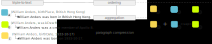
\includegraphics[width=\textwidth]{img/zeroshot_pipeline.pdf}
    \caption{A scheme of our approach for zero-shot data-to-text generation from RDF triples. After a simple transformation of triples to facts, we apply the pipeline of modules for (1) ordering, (2) aggregation, (3) paragraph compression. Individual modules are trained on a large general-domain text corpus and operate over text in natural language. In-domain knowledge is included only in the simple hand-crafted templates for each predicate.}\label{fig:zeroshot:pipeline}
\end{figure}
In this section, we provide the formal description of our proposed approach. Similarly to \Cref{sec:finetuning,sec:iterative}, we focus on the task of producing a natural language description $Y$ a set of \ac{rdf} triples $x \in X$, where each triple $x = (s, p, o)$ describes the relation $p$ between the entities $s$ and $o$ in the knowledge graph.

Our pipeline proceeds as follows. Given a set of triples $X$ on the input, we:
\begin{enumerate}
    \item transform the triples into \textit{facts}, which are short sentences in natural language,
    \item sort the facts using an \textit{ordering} module,
    \item insert sentence delimiters between the sorted facts using an \textit{aggregation} module,
    \item input the ordered sequence of facts with delimiters into a \textit{paragraph compression} module, which generates the final description $Y$.
\end{enumerate}

\paragraph{Transforming Triples to Facts}
\label{sec:templates}
The first step in our pipeline involves transforming each of the input triples $x_i \in X$ into a fact $f_i \in F$  using a transformation $T: X \rightarrow F$. We define a fact $f_i$ as a single sentence in natural language describing $x_i$.
The transformation serves two purposes: (a) preparing the data for the subsequent text-to-text operations, (b) introducing in-domain knowledge about the semantics of individual predicates.


% This step can be realized e.g. using a simple template for each predicate (cf. §\ref{sec:templates_model}).
% Several neural methods for this task were proposed, using either interactions between pairs of sentences \cite{chen2016neural,li2017neural}, global interactions \cite{gong2016end,wang2019hierarchical}, or combination of both \cite{cui2020bert}. We base our ordering module (§\ref{sec:ord_model}) on the recent work of \citet{calizzano2021ordering}, who use a pointer network \cite{wang2019hierarchical,vinyals2015pointer} on top of a PLM.


\paragraph{Ordering} We assume that the default order of triples $X$ is random and the same applies for the respective facts $F$. Note, however, that $F$ is a set of meaningful sentences. We can use this to our advantage and apply a sentence ordering module \cite{barzilay2001sentence,lapata2003probabilistic} to maximize the coherency of the paragraph resulting from their concatenation. An example outcome of such operation may be grouping together facts mentioning \textit{birth date} and \textit{birth place} of a person, followed by their \textit{occupation}, as it is shown in \autoref{fig:zeroshot:pipeline}.

Formally, we apply the ordering module $O(F)$ to get an ordered sequence of facts: $F_o = \{f_{o_1}, \ldots, f_{o_n}\}$, where $o_{1:n}$ is a permutation of fact indices. The ordering module allows downstream modules to only focus on operations over neighboring sentences.


\paragraph{Aggregation} Some facts will be typically mentioned together in a single sentence. Considering the previous example, \textit{occupation} is likely to be mentioned separately, while \textit{birth date} and \textit{birth place} are likely to be mentioned together. Unlike previous works \cite{wiseman2018learning,shao-etal-2019-long,shen-etal-2020-neural,xuAGGGENOrderingAggregating2021}, which capture the segments corresponding to individual parts of the input as latent variables, we simply insert delimiters into the ordered sequence of facts to mark sentence boundaries.

Formally, the aggregation module takes a sequence of ordered facts $F_o$ as input and produces a sequence of sentence delimiters $A(F_o) = \{\delta_{o_1}, \delta_{o_2}, \ldots, \delta_{o_{n-1}}\}$; $\delta_{i} \in \{0, 1\}$. The output $\delta_{i}=1$ means that the neighboring facts should be mentioned separately, i.e. the neighboring sentences should \textit{not} be fused. Conversely, $\delta_{i}=0$ means that the facts should be aggregated and their corresponding sentences should be fused. The markers serve as sentence fusion hints for the paragraph compression module.



\paragraph{Paragraph Compression}  The \ac{pc} module aim to output the final text description.  It has two main objectives: (a) \textit{fusing} related sentences, i.e., sentences $i$ and $j$ in between which $\delta_{i}=0$, and (b) \textit{rephrasing} the text to improve its fluency, e.g. fixing disfluencies in the templates, replacing noun phrases with refering expressions, etc.

Formally, the model takes as input the ordered sequence of facts with delimiters $F_a = \{f_{o_1}, \delta_{o_1}, f_{o_2}, \ldots, \delta_{o_{n-1}}, f_{o_n}\}$ and produces the final text $Y$. Unlike in text summarization or sentence simplification, the edits will typically be minor, since the goal is to preserve the semantics of the already ordered sequence of sentences.



\subsection{\textsc{WikiFluent} Corpus}
\label{sec:pipeline:wikifluent}
Here we descibe the process of building a large-scale synthetic corpus \textsc{WikiFluent}. The corpus provides training data for the neural models which we use in our implementation of the ordering, aggregation, and paragraph compression modules (see \autoref{sec:pipeline:exp}).

Our goal is to cover a broad range of domains while capturing the sentence style in D2T generation with respect to both the input facts and the target descriptions. In other words, we aim to build a corpus in which (1) the input is a set of simple, template-like sentences, (2) the output is a fluent text in natural language preserving the semantics of the input. As we describe below in detail, we achieve that by using human-written paragraphs in English Wikipedia and applying \textit{split-and-rephrase} and  \textit{coreference resolution} models to obtain synthetic source texts. The process is illustrated in Figure \ref{fig:wikifluent}; corpus statistics are included in Appendix \ref{app:stats}.

\subsection{Data Source} For building the \textsc{WikiFluent} corpus, we extracted 934k first paragraphs of articles from a Wikipedia dump\footnote{\texttt{enwiki-20210401-pages-articles-multistream}} using WikiExtractor \cite{Wikiextractor2015}. Wikipedia is commonly used for large-scale pretraining of D2T generation models \cite{jin2020genwiki,chen-etal-2020-kgpt}. Although it is not bias-free, it provides more balanced sample of natural language use than typical D2T generation datasets. We used the first paragraphs of Wikipedia entries, which contain mostly concise, fact-based descriptions.
We selected paragraphs with length between 30-430 characters; filtering out lists, disambiguations, and repeated and malformed paragraphs. To balance the length of inputs, we selected 250k examples each from 4 equally sized length ranges (30-130 characters, etc.).



\begin{figure}[t]
    \centering
    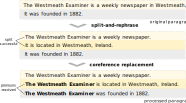
\includegraphics[width=0.5\textwidth]{img/wikifluent.pdf}
    \caption{The building process of the \textsc{WikiFluent} corpus. We apply a split-and-rephrase model on each sentence in the paragraph and resolve coreferences in the split sentences. The result is a set of simple sentences which together convey the same meaning as the original paragraph. The synthesized sentences are used as \textit{input} into our models, the original human-written texts are used as \textit{ground truth}.}\label{fig:wikifluent}
\end{figure}

\paragraph{Split-and-Rephrase}

To generate a set of simple sentences, we divide each paragraph into sentences using NLTK \cite{bird2006nltk} and apply a \textit{split-and-rephrase} model on each sentence. Split-and-rephrase is a task of splitting a complex sentence into a meaning preserving sequence of shorter
sentences \citep{narayan-etal-2017-split}. The process is illustrated in the upper part of Figure \ref{fig:wikifluent}.

We train our split-and-rephrase model on the large-scale WikiSplit corpus by \citet{botha-etal-2018-learning}, containing human-made sentence splits from Wikipedia edit history. Following the same setup as for a paragraph compression model (§\ref{sec:pc}), we train BART-base \cite{lewis2020bart} on the WikiSplit dataset in a sequence-to-sequence setting. Next, we apply the trained split-and-rephrase model on each sentence in our Wikipedia-based corpus, uniformly randomly choosing between 0-2 recursive calls to ensure that the splits are not deterministic. If the sentence cannot be meaningfully split, the model tends to duplicate the sentence on the output; in that case, we use only the original sentence and do not proceed with the splitting.

\paragraph{Coreference Replacement}  As the next step, we concatenate the split sentences and apply a coreference resolution model \cite{gardner2018allennlp,Lee2018HigherorderCR} in order to replace referring expressions with their antencendents (e.g., pronouns with noun phrases). The motivation for this step is to match the style of the facts (see §\ref{sec:templates}), which do not use pronouns since each fact describes a single triple only. Note that this procedure replaces the referring expressions only in the synthesized sentences (which are used as input) and keeps them in the original paragraphs (which are used as ground truth). As a consequence, the paragraph compression module is implicitly trained to generate referring expressions in the final description.

\paragraph{Filtering} To ensure that the generated sentences convey the same semantics as the original paragraph, we use a pretrained RoBERTa model\footnote{\url{https://huggingface.co/roberta-large-mnli}} \cite{liu2019roberta} trained on the MultiNLI dataset \cite{williams2018broad} for checking the semantic accuracy of the generated text. Following \citet{duvsek2020evaluating}, we test if the original paragraph entails each of the synthesized sentences (checking for omissions), and if the set of concatenated synthesized sentences entails the original paragraph (checking for hallucinations). In a filtered version of the \textsc{WikiFluent} corpus, we include only the examples without omissions or hallucinations (as computed by the model), reducing it to 714k examples (approximately 75\% of the original size).

\subsection{Experiments}
\label{sec:pipeline-exp}
% In this paper, we present a \emph{zero-shot} alternative to the traditional finetuning paradigm by formulating the D2T generation from RDF triples as a sequence of general-domain operations over text in natural language. We start by transforming individual triples to text using trivial templates, which we subsequently order, aggregate, and compress on the paragraph level to produce the resulting description of the data. In constrast to traditional pipeline systems, all our pipeline modules are built upon PLMs and operate over sentences in natural language. The modules are trained on our new \textsc{WikiFluent} corpus, which contains 934k examples of first paragraphs from the English Wikipedia, each supplied with a synthesized set of simple template-like sentences which together convey the meaning of the original paragraph.
% Our approach allows generating natural language descriptions from RDF triples with a minimum amount of domain-specific rules or knowledge and without using training data from the D2T datasets. Although our approach is primarily a probe into the territory of zero-shot approaches and cannot yet match the quality of state-of-the-art models, we show that it can yield large improvements upon simple baselines and match older supervised systems on automatic metrics for text fluency. Moreover, the semantic accuracy metrics and our manual error analysis suggest that our approach offers a way to prevent omissions and hallucinations common in few-shot approaches.


\chapter{Evaluating Generated Text}
\label{chap:evaluation}


In this chapter, we introduce two approaches for evaluating semantic accuracy of \ac{d2t} generation.

\section{Evaluating Semantic Accuracy}
\label{sec:sem-acc}

\begin{refbox}
    This section is based on the paper \emph{Evaluating Semantic Accuracy of Data-to-Text Generation with Natural Language Inference} \cite{dusekEvaluatingSemanticAccuracy2020}, joint work with Ondřej Dušek, published in the Proceedings of the The 13th International Conference on Natural Language Generation (INLG 2020). The experimental part was done by Ondřej Dušek, the author of this thesis came up with the initial idea and did the paper writing. The paper has received the award for the best short paper at the conference.
\end{refbox}

We propose a new metric for evaluating the semantic accuracy of D2T generation
based on a neural model pretrained for \ac{nli}. We use the \ac{nli} model to check textual entailment between the input data and the output text in both directions, allowing us to reveal omissions or hallucinations. Input data are converted to text for \ac{nli} using trivial templates. Our experiments on two recent D2T datasets show that our metric can achieve high accuracy in identifying erroneous system outputs. The experimental code for our metric is available on GitHub.\footnote{\url{https://github.com/ufal/nlgi_eval}}

\subsection{Motivation}
State-of-the-art neural \ac{d2t} generation models are prone to omitting or hallucinating facts \cite{gehrmanngehrmannEndtoEndContentPlan2018,ferrferreiraNeuralDatatotextGeneration2019,dusekEvaluatingStateoftheartEndtoEnd2020}, which restricts their real-world deployment. Recognizing these errors is thus essential for
proper system evaluation and further research in D2T generation.

In general, evaluating the semantic accuracy of D2T generation outputs requires full natural language understanding. Minor changes in wording may cause major differences in the meaning of the text, making it difficult for handcrafted heuristics to cover all edge cases. Human evaluation, on the other hand, is expensive and difficult to scale.

We note that the task of checking if a generated sentence includes/entails a particular fact is very close to the task of \ac{nli}. \ac{nli} is a sequence classification task which takes two inputs---a \textit{hypothesis} and a \textit{premise}---and produces one of the possible outputs: the hypothesis is \textit{entailed} by (follows from) the premise, \textit{contradicts} the premise, or their relation is \textit{neutral}. Recently, neural models for \ac{nli} \cite{zhang2019,liu-etal-2019-multi,liu_roberta_2019} reached near-human levels of performance and \ac{nli} was used for evaluating the output of abstractive summarization systems \cite{maynez-etal-2020-faithfulness}.

This brings a question: Can we use an \ac{nli} model for evaluating the semantic accuracy of D2T outputs?
The main idea of our method is to check with a general pretrained \ac{nli} model if the semantic information implied by the input data and the generated text is equal. We achieve this by using the \ac{nli} model to check for \textit{entailment} in two directions: By inferring input facts from the generated text we can check for \textit{omissions}, while the other direction allows us to check for \textit{hallucinations}.\footnote{This check in both directions is appropriate for D2T tasks that do not include content selection, which are the focus of our experiments in this paper. If the generator is supposed to select just some of the input facts to verbalize \cite[cf.~e.g.][]{wiseman_challenges_2017}, we can either only check for hallucinations or, if the content selection is explicit, perform a two-way check with the selected facts provided.}
For instance, consider the two input facts from Figure~\ref{fig:ex}: \emph{(Blue Spice | eat\_type | pub)}, \emph{(Blue Spice | area | riverside)} and the generated text: “You can bring your kids to Blue Spice in the riverside area.” A \ac{nli} system should detect that the first fact is not entailed by the text (there is no mention of Blue Spice being a pub), but the text is also not entailed by the facts (the information about kids is hallucinated).

Applying \ac{nli} for the D2T task brings a problem:
The hypothesis for the standard \ac{nli} task is a natural language text, but the input for D2T generation is structured. However, we show that we can easily sidestep this issue by transforming the data into text using a trivial template for each fact.

We demonstrate that even without any human references or in-domain training and with minimal handcrafting, our approach achieves high accuracy (>90\%) on the E2E Challenge data \cite{duvsek2020evaluating}, competitive with scripts specifically handcrafted for the domain, and produces useful results (>75\% accuracy, 0.6 Spearman correlation with human scores)
on the more challenging WebNLG dataset \cite{gardent2017webnlg}. A manual error analysis shows that some instances marked as errors were in fact assessed correctly by our metric; we also identified a few major sources of errors that can be mitigated by in-domain tuning.

\begin{figure*}[t]
    \centering
    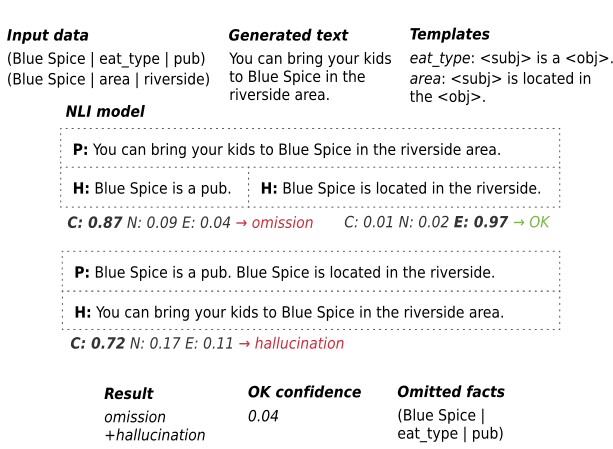
\includegraphics[width=\textwidth]{img/2020_nli_inlg}
    \caption{An example of evaluating the output from a D2T system with our metric. The generated text is used as a \textit{premise} (\textit{P}) to check for omissions and as a \textit{hypothesis} (\textit{H}) to check for hallucinations. The \ac{nli} model generates probabilities for \textit{contradiction} (\textit{C}), \textit{neutral} (\textit{N}) and \textit{entailment} (\textit{E}).}
    \label{fig:sem-acc:ex}
\end{figure*}
\paragraph{Automatic Evaluation of NLG} NLG outputs were traditionally evaluated by reference-based metrics measuring \emph{n}-gram overlap with a reference, such as BLEU \cite{papineni-etal-2002-bleu}, ROUGE \cite{lin-2004-rouge} and METEOR \cite{lavie_meteor:_2007}. Alternative, referenceless quality estimation metrics based on language model scores \cite{kann_sentence-level_2018} or linguistic features \cite{tian_treat_2018} focus on fluency and do not consider semantic accuracy. Recent works try to estimate NLG output quality with finetuned pretrained models \cite{zhou_learning_2020,zhang_bertscore:_2020,sellam_bleurt_2020}. The score from these models can capture some aspects of semantic accuracy, but only implicitly.

\paragraph{Semantic Accuracy}
To our knowledge, there is no generally accepted automatic metric for explicitly measuring semantic accuracy of NLG outputs. The closest commonly used metric is the \textit{slot error rate}, which is typically based on pattern matching tailored for a given dataset \cite{reed-etal-2018-neural,ijcai2019-437,duvsek2020evaluating}. Recently, \citet{goodrich_assessing_2019} introduced a metric based on training a neural model on named-entity recognition and fact extraction.

\paragraph{Faithful NLG}
Some recent neural NLG systems %of the works on neural NLG 
train specifically for semantic accuracy
%aim to make the output more faithful to the input 
\cite{nie-etal-2019-simple,tian2019sticking,kedzie-mckeown-2019-good}. Similarly to us, \citet{harkous2020have} use a pretrained neural model as a classifier to detect inaccurate output, finetuning the classifier on manually augmented domain-specific data.

Unlike previous works, we use a pretrained neural model finetuned for \ac{nli} which we do not further train on any domain-specific data.
\paragraph{Automatic Evaluation of NLG} NLG outputs were traditionally evaluated by reference-based metrics measuring \emph{n}-gram overlap with a reference, such as BLEU \cite{papineni-etal-2002-bleu}, ROUGE \cite{lin-2004-rouge} and METEOR \cite{lavie_meteor:_2007}. Alternative, referenceless quality estimation metrics based on language model scores \cite{kann_sentence-level_2018} or linguistic features \cite{tian_treat_2018} focus on fluency and do not consider semantic accuracy. Recent works try to estimate NLG output quality with finetuned pretrained models \cite{zhou_learning_2020,zhang_bertscore:_2020,sellam_bleurt_2020}. The score from these models can capture some aspects of semantic accuracy, but only implicitly.

\paragraph{Semantic Accuracy}
To our knowledge, there is no generally accepted automatic metric for explicitly measuring semantic accuracy of NLG outputs. % in terms of faithfulness to the input data. 
The closest commonly used metric is the \textit{slot error rate}, %for computing omissions, 
which is typically based on pattern matching tailored for a given dataset \cite{reed-etal-2018-neural,ijcai2019-437,duvsek2020evaluating}. Recently, \citet{goodrich_assessing_2019} introduced a metric based on training a neural model on named-entity recognition and fact extraction.

\paragraph{Faithful NLG}
Some recent neural NLG systems %of the works on neural NLG 
train specifically for semantic accuracy
%aim to make the output more faithful to the input 
\cite{nie-etal-2019-simple,tian2019sticking,kedzie-mckeown-2019-good}. Similarly to us, \citet{harkous2020have} use a pretrained neural model as a classifier to detect inaccurate output, finetuning the classifier on manually augmented domain-specific data.

Unlike previous works, we use a pretrained neural model finetuned for \ac{nli} which we do not further train on any domain-specific data.



\subsection{NLI model}
\label{sec:nli-model}
% No training needed
We use pretrained RoBERTa \cite{liu_roberta_2019} as implemented in the Transformers library \cite{wolf_huggingfaces_2020} for our \ac{nli} model. Specifically, we use the \texttt{roberta-large-mnli}\footnote{\scalebox{0.95}[1.0]{\url{https://huggingface.co/roberta-large-mnli}}} checkpoint, which was finetuned on the Multi\ac{nli} dataset \cite{williams-etal-2018-broad}. We use the model \textit{as is}, without any further training. %on our side.
Given a premise text and a hypothesis text, the \ac{nli} model produces a probability distribution over three results: \textit{contradiction}, % (the hypothesis contradicts the premise), 
\textit{neutral} %(the hypothesis does not contradict, but does not follow from the premise) 
and \textit{entailment} (cf.~Section~\ref{sec:intro}). % (the hypothesis follows from the premise).
We consider a \ac{nli} check as passed if the probability for \textit{entailment} is the highest of the three.

\subsection{Data Preparation}
\label{sec:templates}

% We focus on triple-like MRs, easy to represent others
The input to our metric is a set of facts (the input for a D2T system) and the corresponding verbalization of these facts (the output from a D2T system). In our setup, the facts are RDF-like triples in the \textit{subject-predicate-object} form.%\footnote{This can be easily extended to other similar data formats. (e.g., the E2E dataset was converted from attribute-value pairs for our experiments).}

We convert each triple
to natural language using a trivial template. We consider two cases:
\begin{enumerate}[nosep,label={(\arabic*)},leftmargin=14pt,labelwidth=12pt,labelsep=2pt]
    \item \emph{Default:} The templates can be handcrafted or extracted from the NLG systems' training data for each predicate.
    \item \emph{Backoff:} We use only a single, universal ``backoff'' template for all the facts, in the form: \emph{The \textless{}predicate\textgreater{} of \textless{}subject\textgreater{} is \textless{}object\textgreater{}}.
\end{enumerate}
Hereinafter, a \textit{fact} refers to a template filled with the values from the triple.


\subsection{Evaluation Process}
\label{sec:eval-process}

% Individual triples, take the max, must be E
The generated text is said to be correct if it mentions \textit{all} and \textit{only} the input facts.
We check if the text contains any omissions or hallucinations in two steps (see Figure~\ref{fig:ex} for an example):
\begin{enumerate}[nosep,label={(\arabic*)},leftmargin=14pt,labelwidth=12pt,labelsep=2pt]
    \item To check for omissions, we use the whole generated text as a premise and sequentially feed each fact as a hypothesis to the \ac{nli} model. Any failed \ac{nli} check is considered an omission. While we could use all concatenated facts in a single \ac{nli} check, our approach gives us further information about which facts are omitted.
    \item To check for hallucinations, we use a concatenation of all facts as a premise and feed the generated text as a hypothesis to the \ac{nli} model. If this \ac{nli} check fails, the text is considered to contain hallucination. This step cannot be split into simpler \ac{nli} checks.
\end{enumerate}
The final output of our metric is either 4-way (denoted as \textsc{Fine}): \emph{OK} (i.e., all \ac{nli} checks passed), \emph{omission}, \emph{hallucination} or \emph{omission+hallucination} (based on the failed checks), or 2-way (denoted as \textsc{Rough}) where the latter three results are collapsed into \emph{not\_OK}. The \textsc{Fine} 4-way output is more useful for system evaluation (we can distinguish whether the system tends to hallucinate or omit information). The \textsc{Rough} 2-way output corresponds more to a usage inside an NLG system for output reranking or filtering: any output that is \emph{not\_OK} should be penalized/\hspace{0mm}filtered out.
% Computing confidence: minimum for all
Additionally, we compute a \textit{confidence score} of the model as the minimum of all the entailment probabilities. %This score can serve as a measure of the model's confidence about the correctness of the generated text.


% =============================================================================
\section{Experimental Setup}
\label{sec:experiments}
% -----------------------------------------------------------------------------

% Two prominent recent data-to-text datasets



% Does have some problems, mostly related to domain (not family friendly -!> adult only, some random babble is hallucination...)

We experiment with two recent English data-to-text datasets with a triple-like format: WebNLG \cite{gardent2017webnlg} and E2E \cite{novikova-etal-2017-e2e}.\footnote{E2E data use attribute-value pairs relating to a restaurant; we convert them to triples where the restaurant is the subject.} Since both of them were used in shared tasks, sets of system outputs and measures of semantic accuracy are available (see Supplementary for details).
% Eval on WebNLG human rated, corr with humans
% No binary -> thresholding at 2.5 ()

For WebNLG, we compare our metric with crowdsourced human ratings of semantic adequacy \cite{shimorina2019webnlg}. %In particular, we use the question about semantic adequacy: \textit{Does the text correctly represent the meaning in the data?}, where the 
Human annotators used
%indicated the answer on 
a three-point Likert scale (1 = Incorrect, 2 = Medium, 3 = Correct) and answers are averaged over multiple annotators. In our experiments discussed in Section~\ref{sec:webnlg_results}, we consider a sentence correct if it achieved human rating 2.5 or higher (we also tried a threshold of 2.0, with slightly worse results).
% less accurate on humans
% but still quite OK. Since the domain is quite limited, this is possible to do.

For the E2E dataset, the challenge results were checked for semantic accuracy using a handcrafted automatic script \cite{duvsek2020evaluating},\footnote{While the E2E challenge did include crowdsourced evaluation of semantic accuracy, the results were unreliable, overestimating the number of errors \cite{duvsek2020evaluating}. Note that unlike our metric, such a handcrafted approach to evaluating semantic accuracy is only viable for limited domains such as E2E.%\OD{is the “unlike our metric” OK or too boastful?} \ZK{tak teď už všichni vidí, že se trefuješ sám do sebe, ne? :D mně to přijde ok, akorát je tu na mě moc poznámek pod čarou... co dát poznámku 4 do závorky do textu?}
} we therefore use this automatic script as the ground truth for evaluating our metric in Section~\ref{sec:e2e-results}.
We further use small sets of system outputs and human-written texts with expert annotation \citep[provided by][]{dusek_semantic_2019} to evaluate our approach against gold-standard annotation and to compare to existing semantic accuracy classifiers for E2E data in Section~\ref{sec:e2e-classifiers}.


We evaluate the \emph{Default} and \emph{Backoff} approaches to acquiring templates as described in Section~\ref{sec:templates}. The \emph{Default} setup works with one custom template per predicate type. For WebNLG, we obtained templates by delexicalizing human references for single-triple examples from WebNLG training data.\footnote{For each predicate, we choose randomly if more templates are found and use the backoff if no templates are found.} For E2E, we handcrafted 8 templates.
The templates are filled with values from individual input triples and concatenated for multi-triple inputs as described in Section~\ref{sec:eval-process}. %\OD{is this OK? they're not concatenated for omission checks; OTOH R\#1 didn't really get this and thought we can only handle 1-triple WebNLG stuff} \ZK{jo, myslím, že je to takhle pochopitelný}


% There's also limited human-annotated system outputs (400) and human-written scripts (200),
% where we can compare to the automatic script.

% =============================================================================
\section{Results Analysis}
\label{sec:results}
% -----------------------------------------------------------------------------


\begin{table}[t]
    \centering \small
    \begin{tabular}{l ccccc} \toprule
                & \textbf{A} & \textbf{R} & \textbf{P} & \textbf{F1} & $\mathbf{\rho}$ \\\midrule
        Default & 0.775      & 0.772      & 0.796      & 0.784       & 0.628           \\
        Backoff & 0.768      & 0.760      & 0.793      & 0.776       & 0.637           \\ \bottomrule
    \end{tabular}
    \caption{WebNLG dataset results, compared to crowdsourced human ratings (A = accuracy, R = recall, P = precision, F1 = F-measure, $\rho$ = Spearman correlation of confidence scores with human scores).}
    \label{tab:webnlg}
\end{table}

\begin{table}[t]
    \centering \small
    \begin{tabular}{l cccccc} \toprule
                & \textbf{Af} & \textbf{Ar} & \textbf{R} & \textbf{P} & \textbf{F1} \\\midrule
        Default & 0.911       & 0.933       & 0.895      & 0.910      & 0.903       \\
        Backoff & 0.846       & 0.874       & 0.913      & 0.768      & 0.834       \\
        \bottomrule
    \end{tabular}
    \caption{E2E dataset results, compared to the automatic evaluation script %The experiments on the second lines ignore \textit{eatType=restaurant}. 
        (Af = \textsc{Fine} accuracy, Ar = \textsc{Rough} accuracy, R = recall, P = precision, F1 = F-measure).}
    \label{tab:e2e}
\end{table}


\begin{table*}[t]
    \centering\footnotesize
    \begin{tabular}{@{}l c c ccc >{\hspace{3mm}} c c ccc@{}}\toprule
                          & \multicolumn{5}{c}{\bfseries Human-written (E2E training set)} & \multicolumn{5}{c}{\bfseries System outputs (TGen)}                                                                     \\
                          & \bf Af                                                         & \bf Ar                                              & \bf R & \bf P & \bf F1 & \bf Af & \bf Ar & \bf R & \bf P & \bf F1 \\\midrule
        Slug2Slug aligner & 0.685                                                          & 0.765                                               & 0.550 & 0.800 & 0.652  & 0.995  & 1.000  & 1.000 & 1.000 & 1.000  \\
        %                              & 0.920 & 0.930 & 0.977 & 0.764 & 0.857 & 0.990 & 0.995 & 1.000 & 0.947 & 0.973 \\
        E2E script        & 0.820                                                          & 0.885                                               & 1.000 & 0.777 & 0.874  & 0.995  & 0.995  & 1.000 & 0.950 & 0.974  \\
        %                              & 0.615 & 0.700 & 1.000 & 0.417 & 0.589 & 0.990 & 0.990 & 1.000 & 0.900 & 0.947 \\
        TGen reranker     & 0.110                                                          & 0.435                                               & 0.975 & 0.413 & 0.579  & 0.220  & 0.278  & 1.000 & 0.116 & 0.208  \\
        %                              & 0.100 & 0.270 & 1.000 & 0.228 & 0.371 & 0.218 & 0.273 & 1.000 & 0.110 & 0.198 \\ 
        \midrule
        % TGen rer. cls. (cleaned data) & 0.155 & 0.415 & 0.988 & 0.405 & 0.574 & 0.338 & 0.403 & 1.000 & 0.138 & 0.241 \\
        %   & 0.100 & 0.240 & 1.000 & 0.221 & 0.361 & 0.338 & 0.398 & 1.000 & 0.130 & 0.230 \\\midrule
        Default           & 0.600                                                          & 0.700                                               & 0.625 & 0.625 & 0.625  & 0.978  & 0.978  & 0.947 & 0.837 & 0.888  \\ % 005
        %                              & 0.765 & 0.805 & 0.976 & 0.525 & 0.683 & 0.983 & 0.983 & 1.000 & 0.837 & 0.911 \\ % 007
        Backoff           & 0.530                                                          & 0.640                                               & 0.675 & 0.540 & 0.600  & 0.833  & 0.833  & 0.974 & 0.359 & 0.525  \\\bottomrule % 006
        %                              & 0.665 & 0.705 & 0.977 & 0.420 & 0.587 & 0.835 & 0.835 & 1.000 & 0.353 & 0.522 \\\bottomrule % 008
    \end{tabular}
    \caption{Semantic classifiers evaluated on expert human annotation on E2E data (see Table~\ref{tab:e2e} for metrics legend).} %; second line ignores eatType=restaurant}
    \label{tab:e2e-slot-comparison}
\end{table*}



% Random baseline would be 0.5 or 0.25 for fine
We evaluate our metric in terms of accuracy, precision, recall, and F1-measure (where \emph{not\_OK} samples are treated as positive since we focus on detecting errors).
We additionally perform a manual error analysis on a random sample of 100 error examples for each dataset, i.e.\ examples where our metric gave a different assessment from the ground truth (provided by crowdsourced annotation for WebNLG and by a handcrafted classification script for E2E as described in Section~\ref{sec:experiments}). % \ZK{zase bych dal poznámku klidně do textu, ať čtenář nemusí tolik skákat}
In general, the results are high above the random baseline (0.5 for the \textsc{Rough} metric and 0.25 for the \textsc{Fine} metric) but differ between the datasets, which we discuss below. %in the following subsections.



% The results for the E2E dataset are better, probably due to the lower lexical variability of the dataset.
% \OD{a možná kvůli tomu, že human eval pro webnlg je trochu zašuměný, ale nevim, jestli se to sem hodí}


% recall is probably more important than precision (not that there are differences)

\subsection{WebNLG Analysis}
\label{sec:webnlg_results}
The overall scores for the WebNLG dataset are summarized in Table \ref{tab:webnlg}. %Here, we compare the \textsc{Rough} metric against the (thresholded) human rating.
To further check whether the size of the input affects performance, we computed Spearman correlation of the number of input triples with metric errors. The resulting very low value of -0.05 ($p=$\,0.02, \emph{Default} setting) shows that the metric holds its performance even for more complex WebNLG examples. %\OD{added this, does it work here?} \ZK{chvilku mi trvalo pochopit, co to číslo počítá, ale asi jo}
%\OD{number of predicates doesn't seem to have a huge effect on performance (1: 78.22, 2: 84.00, 3: 73.55, 4: 77.55, 3: 73.95; spearman -0.0503, p=0.0175)}

%
%
% WebNLG much worse, although still better than random
% not much difference with the backoff templates -- 0.77 vs 0.76
% good correlation with human judgements 0.62-0.63
%
% We can see that the setup using only a backoff template leads to almost the same results as the default setup.
%
%\OD{TODO supplementary should have examples}
%\OD{not much difference w.r.t. backoff means templates are bad}
On the other hand, the overall scores show that our metric deviates quite a lot from the human judgments. Our manual error analysis indicates several reasons for that (see Supplementary for examples): (1) The annotation is somewhat noisy and using a threshold is not ideal---many correctly rendered outputs do not reach the 2.5 threshold (while some incorrect ones do). (2) Imprecise templates can confuse the \ac{nli}
%make the metric check for different information 
(e.g., for the predicate \emph{nationality}, our extracted template is \emph{\textless{}subj\textgreater{} was \textless{}obj\textgreater{}}, which works well with values such as \emph{French}, but not with \emph{United States}). This is currently a weak point of our metric, as illustrated by the very small performance difference between the \emph{Default} and \emph{Backoff} setups; however, the issue can be mitigated by a better selection of the templates from training data, e.g.\ using language-model scoring.
(3) The human annotators tend to give lower scores to accurate but ungrammatical or poorly organized texts. Our metric tends to rate these texts as \emph{OK}.
%Third, we note that many examples are dubious, e.g. there are typos in the text or the text interprets the data too loosely. In these cases, the notion of semantic accuracy can differ between the annotators.
Overall, our re-examination shows that almost half of the error examples (42 out of 100) were in fact correctly classified by our metric (i.e.\ their crowdsourced human annotation was incorrect), %\ZK{přidat něco jako "and not by human evaluators", ať je z toho jasný, že se díváme na chyby a tvrdíme, že to vlastně nejsou chyby?}\OD{takhle dobrý?}
so the true performance is most likely higher than the reported numbers. % due to errors in human annotation.

The Spearman correlation of our model's confidence scores with the average human scores is around 0.63 ($p<$1e-10). This is similar to n-gram-based metrics on this data (\citealp{shimorina_human_2018} reports 0.59 for BLEU and 0.73 for METEOR), but unlike these metrics, our approach does not require human-written reference texts.



\subsection{E2E Analysis}
\label{sec:e2e-results}

% E2E -- very good result -- 0.9 rough, 0.92 fine

% below average prices =~ less than £20
% adult only != not family friendly

% noticeable difference w.r.t. backoff templates

The results for the E2E dataset (shown in Table \ref{tab:e2e}) are very good compared to the WebNLG dataset, with over 90\% agreement with the handcrafted script. This can be attributed to lower lexical variability and less noisy texts, as well as to the better quality of the handcrafted templates (the difference between the \emph{Default} and \emph{Backoff} setups is much more pronounced here).
Again, we observe only a very slight drop in performance for more complex E2E inputs (Spearman correlation of metric errors with the number of input triples is -0.08, $p<$1e-10 for the \emph{Default} setting).
%\OD{only slight drop in performance for more complex inputs (around 96\% rough for up to 5 triples, 93\% for 6 triples, 91\% for 7, spearman 0.07638, p=1.3948e-18)}

%The reference texts often ignore \textit{eatType=restaurant}, which is probably deemed as implicit for the domain. We report the results where we ignore this particular slot-value pair and we observe notable improvements.
%\OD{TODO remove this, incl. from tables}
%\OD{TODO bigger diff w.r.t. backoff, i.e. templates are better}
The main issues identified by our error analysis are:
(1) Problems in the interpretation of some values, e.g., \textit{price range=less than \textsterling{}20} is verbalized as ``cheap'' or \textit{family-friendly=no} as ``adult-only''. These cases are classified as \emph{not\_OK} by the \ac{nli} model.
(2) Missing or over-greedy patterns in the slot error script, causing annotation errors.
(3) Edge cases: some expressions cannot be interpreted in a straightforward way, e.g.\ ``high restaurant'' for \emph{pricerange=high} is deemed OK by the \ac{nli} but not by the slot error script.
(4) Expressions in the outputs that do not correspond to input facts, such as ``with full service'', are considered hallucinations by the \ac{nli}, but ignored by the slot error script.
Again, we consider about half of the error examples (45 out of 100) as correctly classified by our metric (see Supplementary for details), and thus our metric's performance is probably higher than the reported values due to erroneous annotation from the handcrafted script.

% - - - - - - - - - - - - - - - - - - - - - - - - - - - - - - - - - - - - - -
\subsection{E2E MR Classifier Comparison}
% - - - - - - - - - - - - - - - - - - - - - - - - - - - - - - - - - - - - - -
\label{sec:e2e-classifiers}
%As described in Section~\ref{sec:experiments}, there are data in the E2E restaurant domain human-annotated for accuracy (part of the training set, some TGen outputs; \citealp{dusek_semantic_2019}). 
We used expert-annotated E2E data samples (%part of the training set and some system outputs, 
cf.~Section~\ref{sec:experiments}) to compare our approach to other accuracy classifiers in the E2E domain:
\begin{itemize}[nosep,leftmargin=10pt]
    \item \textbf{Slug2Slug slot aligner} \citep{juraska_deep_2018} is based on keyword matches. It is carefully tuned but not designed to detect hallucination; it only checks for presence of facts from the input MR.
    \item \textbf{E2E slot error script} (used in Section~\ref{sec:e2e-results}) is based on regular expressions; it is also able to detect irrelevant facts.
    \item \textbf{TGen reranker} is an LSTM-based model trained on the E2E training data to rerank outputs of the TGen system \cite{dusek_sequence--sequence_2016} based on their semantic accuracy.
          % \item TGen's reranking classifier trained on cleaned E2E data (i.e., reclassified by the slot error script)
\end{itemize}

The results for all classifiers (in Table~\ref{tab:e2e-slot-comparison}) are much weaker on human-written data, which exhibit much more variability than system outputs.
%While the TGen reranker may be useful for relative comparisons of system outputs, it 
The TGen reranker is very weak when required to detect all facts properly.
Our approach is slightly less precise than both handcrafted scripts, but the difference is small on system outputs (97.8\% vs. 99.5\% accuracy). If we disregard the value \emph{eatType=restaurant}, which is generally noisy, we get 76.5\% accuracy and 97.6\% recall on the human-written data. Moreover, our approach requires much less handcrafting and is more general.


\section{Token-Level Error Detection}
\label{sec:eval-token}
\subsection{Shared Task}
\label{sec:eval-st}
\subsection{Our Submission}
\label{sec:eval-ours}

\chapter{Data Processing and Visualization}
\label{chap:tabgenie}
% \section{Motivation}
% \label{sec:data-mot}
\section{TabGenie Toolkit}
\label{sec:tabgenie}

\begin{refbox}
    This section is based on the paper \emph{\textsc{TabGenie}: A Toolkit for Table-to-Text Generation} \cite{kasnerTabGenieToolkitTabletoText2023}, joint work with Ekaterina Garanina, Ondřej Plátek, and Ondřej Dušek. The work was published as a system demonstration in the Proceedings of the 61st Annual Meeting of the Association for Computational Linguistics (ACL 2023). The project was led by the author of the thesis, the remaining authors helped with implementing the framework and paper writing.
\end{refbox}

Heterogenity of data-to-text generation datasets limits the research on data-to-text generation systems. We present \textsc{TabGenie} -- a toolkit which enables researchers to explore, preprocess, and analyze a variety of data-to-text generation datasets through the unified framework of \textit{table-to-text generation}. In \textsc{TabGenie}, all inputs are represented as tables with associated metadata. The tables can be explored through a web interface, which also provides an interactive mode for debugging table-to-text generation, facilitates side-by-side comparison of generated system outputs, and allows easy exports for manual analysis. Furthermore, \textsc{TabGenie} is equipped with command line processing tools and Python bindings for unified dataset loading and processing. We release \textsc{TabGenie} as a PyPI package\footnote{\url{https://pypi.org/project/tabgenie/}} and provide its open-source code and a live demo at \url{https://github.com/kasnerz/tabgenie}.

Building and evaluating data-to-text (D2T) generation systems \cite{gatt2018survey,sharma2022innovations} requires understanding the data and observing system behavior. It is, however, not trivial to interact with the large volume of D2T generation datasets that have emerged in the last years (see Table~\ref{tab:datasets}).
Although research on D2T generation benefits from platforms providing unified interfaces, such as HuggingFace Datasets \cite{lhoest2021datasets} or the GEM benchmark \cite{gehrmann2021gem}, these platforms still leave the majority of the data processing load on the user.

A key component missing from current D2T tools is the possibility to visualize the input data and generated outputs. Visualization plays an important role in examining and evaluating scientific data \cite{Kehrer2013VisualizationAV} and can help D2T generation researchers to make more informed design choices. A suitable interface can also encourage researchers to step away from unreliable automatic metrics \cite{gehrmann2022repairing} and focus on manual error analysis \cite{van_miltenburg_underreporting_2021,van_miltenburg_barriers_2023}.

Along with that, demands for a \textit{unified input data format} have recently been raised with multi-task training for large language models (LLMs) \citep[\textit{inter alia}]{Sanh2021MultitaskPT,scao2022bloom,Ouyang2022TrainingLM}. Some works have used simple data linearization techniques for converting structured data to a textual format, in order to align it with the format used for other tasks \cite{UnifiedSKG,tang2022mvp}. However,  linearizations are using custom preprocessing code, leading to discrepancies between individual works.


In this paper, we present \textsc{TabGenie} -- a multi-purpose toolkit for interacting with D2T generation datasets and systems designed to fill these gaps. On a high level, the toolkit consists of (a) an interactive web interface, (b) a set of command-line processing tools, and (c) a set of Python bindings (see Figure~\ref{fig:teaser}).


The cornerstone of \textsc{TabGenie} is a \textbf{unified data representation}. Each input represented is as a matrix of $m$ columns and $n$ rows consisting of individual cells accompanied with metadata (see §\ref{sec:data}). Building upon this representation, \textsc{TabGenie} then provides multiple features for unified workflows with table-to-text datasets, including:
\begin{enumerate}
    \item visualizing individual dataset examples in the tabular format (§\ref{sec:exploration}),
    \item interacting with table-to-text generation systems in real-time (§\ref{sec:interactive}),
    \item comparing generated system outputs (§\ref{sec:interactive}),
    \item loading and preprocessing data for downstream tasks (§\ref{sec:python}),
    \item exporting examples and generating spreadsheets for manual error analysis (§\ref{sec:cli}).
\end{enumerate}

In §\ref{sec:casestudies}, we present examples of practical use-cases of \textsc{TabGenie} in D2T generation research.

\subsection{Data}
\label{sec:tabgenie:data}
We currently include 16 datasets listed in Table~\ref{tab:datasets} in \textsc{TabGenie}, covering many subtasks of D2T generation. All the datasets are available under a permissive open-source license.

\begin{figure*}[t]
    \centering
    \setlength{\fboxsep}{0pt}\fcolorbox{gray!20}{white}{\includegraphics[width=1.0\textwidth]{img/tabgenie_web.png}}
    \caption{The web interface of \textsc{TabGenie}. The \textbf{left panel} and the \textbf{navigation bar} contains user controls; the \textbf{center panel} shows table properties and table content; the \textbf{right panel} contains system outputs.}
    \label{fig:web}
\end{figure*}


\subsection{Data Format}
The inputs in D2T generation datasets may not consist only of tables, but also of e.g.\ graphs or key-value pairs. However, we noticed that in many cases, converting these formats to tables requires only minimal changes to the data structure while allowing a unified data representation and visualization. This conversion narrows down the task of D2T generation as the task of generating description for a tabular data, i.e. table-to-text generation \cite{parikh2020totto, liu2022plog, gong2020tablegpt}.


In our definition, a \textit{table} is a two-dimensional matrix with $m$ columns and $n$ rows, which together define a grid of $m \times n$ cells. Each cell contains a (possibly empty) text string. A continuous sequence of cells $\{c_{i}, \ldots, c_{i+k}\}$ from the same row or column may be merged, in which case the values of $\{c_{i+1},\ldots,c_{i+k}\}$ are linked to the value of $c_{i}$.  A cell may be optionally marked as a \textit{heading}, which is represented as an additional property of the cell.\footnote{The headings are typically located in the first row or column, but may also span multiple rows or columns and may not be adjacent.} To better accommodate the format of datasets such as ToTTo \cite{parikh2020totto} or HiTab \cite{cheng2021hitab}, we also allow individual cells to be \textit{highlighted}. Highlighted cells are assumed to be preselected for generating the output description.


The tables may be accompanied with an additional set of properties (see Figure~\ref{fig:web}) -- an example of such a property is a \textit{``title''} of the table in WikiBio \cite{lebret2016neural} or a \textit{``category''} in WebNLG \cite{gardent2017webnlg}. We represent properties as key-value pairs alongside the table. The properties may be used for generating the table description.

\paragraph{Data Transformation}
We aim to present the data as true to the original format as possible and only make some minor changes for datasets which do not immediately adhere to the tabular format:

\begin{itemize}
    \item For graph-to-text datasets, we format each triple as a row, using three columns labeled \textit{subject}, \textit{predicate}, and \textit{object}.
    \item For key-value datasets, we use two columns with keys in the first column as row headings.
    \item For SportSett:Basketball \cite{thomson-etal-2020-sportsett}, we merge the \textit{box score} and \textit{line score} tables and add appropriate headings where necessary.
\end{itemize}

Moreover, for ToTTo \citep{parikh2020totto}, we also provide our custom, improved header cells highlighting (details are given in Appendix \ref{appendix:totto_highlights}).


\paragraph{Data Loading}
To ease the data distribution, we load all the datasets using the Huggingface \texttt{datasets} package \cite{lhoest2021datasets}, which comes equipped with a data downloader. Out of 16 datasets we are using, 7 were already available in Huggingface datasets, either through the GEM benchmark \cite{gehrmann2021gem} or other sources. We publicly added the 9 remaining datasets (see Table~\ref{tab:datasets}).


\textsc{TabGenie} also supports adding custom data loaders. Creating a data loader consists of simple sub-classing the data loader class and overriding a single method for processing individual entries, allowing anyone to add their custom dataset.

\subsection{Web Interface}
\label{sec:tabgenie:web}

\textsc{TabGenie} offers a user-friendly way to interact with table-to-text generation datasets through the \textit{web interface}. The interface can be rendered using a local server (cf. §\ref{sec:cli}) and can be viewed in any modern web browser. The interface features a simple, single-page layout, which contains a navigation bar and three panels containing user controls, input data, and system outputs (see Figure \ref{fig:web}). Although the interface primarily aims at researchers, it can be also used by non-expert users.



\paragraph{Content Exploration}
\textsc{TabGenie} renders input data as HTML tables. This approach provides superior visualizations to existing data viewers, especially in the case of large and hierarchical tables.\footnote{Compare, e.g., with the ToTTo dataset in Huggingface Datasets for which the table is provided in a single field called \textit{``table''}: \url{https://huggingface.co/datasets/totto}}

In the web interface, users can navigate through individual examples in the dataset sequentially, access an example using its index, or go to a random example. The users can add notes to examples and mark examples as favorites for accessing them later. The interface also shows the information about the dataset (such as its description, version, homepage, and license) and provides an option to export the individual examples (see §\ref{sec:cli}).



\paragraph{Interactive Mode}
\textsc{TabGenie} offers an \textit{interactive mode} for generating an output for a particular example on-the-fly. The user can highlight different cells, edit cell contents, and edit parameters of the downstream processor. For example, the user can prompt a LLM for table-to-text generation and observe how it behaves while changing the prompt.

The contents of a table are processed by a processing \textit{pipeline}. This pipeline takes table contents and properties as input, processes them with a sequence of modules, and outputs HTML code. The modules are custom Python programs which may be re-used across the pipelines.

\textsc{TabGenie} currently provides two basic pipelines: (1) calling a generative language model through an API with a custom prompt, and (2) generating graph visualizations of RDF triples. We describe a case-study for the model API pipeline in §\ref{sec:cs:prompting}. Users can easily add custom pipelines by following the instructions in the project repository.

\paragraph{Pre-generated Outputs}
In addition to interactive generation, \textsc{TabGenie} allows users to visualize static pre-generated outputs. These are loaded in the JSONL\footnote{\url{https://jsonlines.org}} format from a specified directory and displayed similarly to model-generated outputs from the interactive mode. Multiple outputs can be displayed alongside a specific example, allowing to compare outputs from multiple systems.


\subsection{Developer Tools}
\label{sec:tabgenie:developer}

\textsc{TabGenie} also provides a developer-friendly interface: Python bindings (§\ref{sec:python}) and a command-line interface (§\ref{sec:cli}). Both of these interfaces aim to simplify dataset preprocessing in downstream tasks. The key benefit of using \textsc{TabGenie} is that it provides streamlined access to data in a consistent format, removing the need for dataset-specific code for extracting information such as table properties, references, or individual cell values.



\paragraph{Python Bindings}
\textsc{TabGenie} can be integrated in other Python codebases to replace custom preprocessing code. With a \textit{single unified interface} for all the datasets, the \textsc{TabGenie} wrapper class allows to:
\begin{itemize}
    \item load a dataset from the Huggingface Datasets or from a local folder,
    \item access individual table cells and their properties,
    \item linearize tables using pre-defined or custom functions,
    \item prepare the Huggingface \texttt{Dataset} objects for downstream processing.
\end{itemize}
\textsc{TabGenie} can be installed as a Python package, making the integration simple and intuitive.
See §\ref{sec:cs:generation} for an example usage of the \textsc{TabGenie} Python interface.


\paragraph{Command-line Tools}
\textsc{TabGenie} supports several basic commands via command line.

\paragraph{Run} The \texttt{tabgenie run} command launches the local web server, mimicking the behavior of \texttt{flask run}. Example usage:

\begin{python}
    tabgenie run --port=8890 --host="0.0.0.0"
\end{python}

\paragraph{Export} The \texttt{tabgenie export} command enables batch exporting of the dataset. The supported formats are \texttt{xlsx}, \texttt{html}, \texttt{json}, \texttt{txt}, and \texttt{csv}. Except for \texttt{csv}, table properties can be exported along with the table content. Example usage:

\begin{python}
    tabgenie export --dataset "webnlg" \
    --split "dev" \
    --out_dir "export/datasets/webnlg" \
    --export_format "xlsx"
\end{python}
\noindent Export can also be done in the web interface.

\paragraph{Spreadsheet} For error analysis, it is common to select $N$ random examples from the dataset along with the system outputs and manually annotate them with error categories (see~§\ref{sec:cs:analysis}). The \texttt{tabgenie sheet} command generates a suitable spreadsheet for this procedure. Example usage:

\begin{python}
    tabgenie sheet --dataset "webnlg" \
    --split "dev" \
    --in_file "out-t5-base.jsonl" \
    --out_file "analysis_webnlg.xlsx" \
    --count 50
\end{python}



\chapter{Data-to-Text Generation with Custom Datasets}
\label{chap:investigating}

In this chapter, we observe and quantify behaviors of neural \acp{lm} in specific \ac{d2t} generation scenarios. To support our investigations, we venture beyond existing \ac{d2t} generation datasets.
% There are several reasons why existing datasets may not be adequate: low variability of data labels, inadequate formats, or the issues with data contamination. 
Building custom datasets helps us to overcome limitations of existing datasets and provide a more detailed picture for the task we set out to study.

In \autoref{sec:rel2text}, we examine the capabilities of \acp{plm} to describe relations between entities in knowledge graphs. As we note, existing datasets were not able to discern memorization from generalization. We thus collect a custom dataset with a large variety of relation labels, including unseen labels in the test set. Using our dataset, we investigate whether the models can correctly describe the relations they have not seen in the training data. We find out that the models can generalize unseen labels as long as the labels are human-readable and unambiguous, which is often (but not always) fulfilled in real-world data.

In \autoref{sec:quintd}, we investigate abilities of open \acp{llm} for \ac{d2t} generation. To prevent data contamination, we scrape unlabeled data from public sources across five domains. As the data is in common formats that the models have seen during pretraining, we can evaluate the ability of the models to describe the data in zero-shot settings. Using \ac{llm}-based referenceless metric and human annotators, we quantify the semantic accuracy of the generated texts with respect to the input data. We find out that although the descriptions are fluent, large majority of them contains semantic errors. We also provide practical recommendations for \ac{d2t} generation in similar scenarios.

\section{Describing Relations in Knowledge Graphs}
\label{sec:rel2text}
\begin{refbox}
    This section is based on the paper \emph{Mind the Labels: Describing Relations in Knowledge Graphs With Pretrained Models} \cite{kasnerMindLabelsDescribing2022}, joint work with Ioannis Konstas and Ondřej Dušek. The work was published in the Proceedings of the 17th Conference of the European Chapter of the Association for Computational Linguistics (EACL 2023). The project was led by the author of the thesis; Ioannis Konstas and Ondřej Dušek mentored the project.
\end{refbox}
In this section, we investigate to which extent do human-readable data labels help \acp{plm} with \ac{d2t} generation. We start by noticing that \acp{plm} can use labels such as column headings, keys, or relation names to generalize to out-of-domain examples. The question is (a) whether this ability robust enough and (b) how accurate are the outputs in cases where these labels are ambiguous or incomplete. To answer this question, we focus on the task of descibing a relation between two entities. For our experiments, we collect \textsc{Rel2Text}: a novel dataset for verbalizing a diverse set of 1,522 unique relations from three large-scale knowledge graphs (Wikidata, DBPedia, YAGO). We evaluate model outputs on unseen relations using a combination of automatic metrics and manual analysis. We find that although \acp{plm} for D2T generation expectedly fail on unclear cases, models trained with a large variety of relation labels are surprisingly robust in verbalizing novel, unseen relations. We argue that using data with a diverse set of clear and meaningful labels is key to training D2T generation systems capable of generalizing to novel domains. We release the code and data for our experiments on Github.\footnote{\url{https://github.com/kasnerz/rel2text}}


% 
% In this paper, 

\subsection{Motivation}
\ac{d2t} generation systems need to accurately capture the semantics of relations between values in the data. However, the data labels such as relation names \cite{farber2018linked,haller2022analysis}, table headings \cite{parikhToTToControlledTableToText2020}, or meaning representation keys \cite{dusekEvaluatingStateoftheartEndtoEnd2020} may provide only superficial or---if the labels are abbreviations, such as in the Rotowire dataset \cite{wiseman2017challenges}---no usable hints about the data semantics.


% \begin{figure}[t]

\begin{table}[t!] \small
    \centering
    \begin{tabular}{llp{3.7cm}l} \toprule
        \textbf{label}    & \textbf{property id}                                       & \textbf{verbalization}                                               & \textbf{note}                       \\ \midrule
        \textit{part of}  & \href{https://www.wikidata.org/wiki/Property:P361}{P361}   & \eh{} is part of \et{}.                                              & can be used verbatim                \\\cdashlinelr{1-4}
        \textit{duration} & \href{https://www.wikidata.org/wiki/Property:P2047}{P2047} & \eh{} lasted for \et{}.                                              & unambiguous verbalization           \\\cdashlinelr{1-4}
        \textit{platform} & \href{https://www.wikidata.org/wiki/Property:P400}{P400}   & \eh{} is available on \et{}.\newline\eh{} runs on \et{}.             & multiple equivalent lexical choices \\\cdashlinelr{1-4}
        \textit{occupant} & \href{https://www.wikidata.org/wiki/Property:P466}{P466}   & \et{} is occupied by \eh{}.\newline\eh{} plays at \et{}.             & semantics depends on entities       \\\cdashlinelr{1-4}
        % \textit{country}  & \href{https://www.wikidata.org/wiki/Property:P17}{P17}     & \eh{} was born in \et{}. \newline \eh{} is located in \et{}.         & semantics depends on entities       \\\cdashlinelr{1-4}
        \textit{parent}   & \href{https://www.wikidata.org/wiki/Property:P8810}{P8810} & \eh{} is the parent of \et{}. \newline \et{} is the parent of \eh{}. & ambiguous relation direction        \\\bottomrule
    \end{tabular}
    \captionof{table}{Example relation labels and the variability in their verbalizations. \eh{} and \et{} denote subject and object in the triple, respectively. The Wikidata page for each relation is available at \url{https://www.wikidata.org/wiki/Property:<property_id>}.}
    \label{tab:rel2text:example}
\end{table}

\acp{plm} such as BART \cite{lewisBARTDenoisingSequencetoSequence2019} or T5 \cite{raffelExploringLimitsTransfer2019} can quickly adapt to new domains and exhibit robustness to out-of-domain inputs. We investigate to what extent are \acp{plm} limited by the expressivity of the data labels. A suitable testing ground is the task of describing individual \acs{rdf}\glsunset{rdf} triples in a \ac{kg}, as shown in \autoref{tab:rel2text:example}. In this task, there is a wide range of lexical choices for the relation label, while the entities can be copied verbatim or with only minor morphological changes. To illustrate the problem, consider the last example in \autoref{tab:rel2text:example}: the model can use its representation of \emph{``parent''} to understand there is a \emph{``is-a-parent-of''} relation between the entities, but it has to infer (or guess) who is the parent of whom. Even in less ambiguous cases, the model still has to correctly capture the intended semantics of the relation (e.g. \emph{``occupant''} meaning \emph{``home team''}).


Current human-annotated datasets for \ac{d2t} generation are not suitable for investigating this problem, as they contain only a small number of relations and rarely contain any unseen relations in the test set \cite{mille2021automatic}. The only existing datasets covering verbalizations of a wider range of \ac{kg} relations are based on \emph{model-generated outputs} \cite{agarwalKnowledgeGraphBased2021,amaral2022wdv}.

We would also like to investigate whether incorporating long-form \emph{descriptions} of data labels helps improving model outputs. Previous works have reach contradictory conclusions: \citet{wang2021kepler} use descriptions of relations instead of their labels for relation embeddings, concluding that it results in worse performance on downstream tasks. Conversely, \citet{kale-rastogi-2020-template} and \citet{lee2021dialogue} improve the performance of their systems by including schema descriptions on the input for the dialogue state tracking and dialogue response generation systems.

Lastly, \emph{verbalizing single triples} is interesting as a stand-alone task. As we have shown previously (\Cref{sec:iterative,sec:pipeline,sec:sem-acc}), in line with other works \cite{xiangASDOTAnyShotDatatoText2022,kale-rastogi-2020-template,gupta2020infotabs,neeraja2021incorporating}, transforming triples to text helps to make the input similar to the format used during pretraining of \acp{plm}. In turn, the transformation helps with applying \acp{plm} on downstream tasks. Various methods have been tried for converting individual triples to text, ranging from simple templates and rule-based systems to prompting \acp{plm}; however, none of these works investigate how to apply these approaches to novel relations.


% 

% Using the \textsc{Rel2Text} dataset, we evalute the ability of \acp{plm} to verbalize relations which were not present in the training set. We consider both models finetuned on other relations in our dataset and models finetuned on datasets from a related domain. We also experiment with scenarios involving few-shot finetuning, training on masked labels, and extending the labels with descriptions (§\ref{sec:analysis},~\ref{sec:results}).

% We find that the \acp{plm} are quite robust in verbalizing a diverse set of relations based on their label (achieving \textasciitilde 90\% of overall entailment probability). We show that semantically unfaithful model outputs are often caused by incomplete, ambiguous, or noisy input data.



% Somewhat suprisingly, we also show that longer relation descriptions do not provide substantial improvements over using short labels.  

% However, even for data using short relation labels, the model trained on verbalizing relations can achieve results comparable to verbalizing relations using manual templates in two downstream tasks (§\ref{sec:downstream}).



\subsection{\textsc{Rel2Text} dataset}
\label{sec:rel2text:data}


For our experiments, we need data with diverse labels and their human verbalizations. We start by collecting a wide set of relations naturally occuring in three large-scale \acp{kg} (Wikidata, DBPedia, and YAGO). For each relation, we collect its label, textual description, and up to five triples in which the relation occurs in the \ac{kg}. We then use human annotatators to collect a \emph{verbalization} for each triple, i.e., a short sentence capturing the meaning of the triple. After filtering, our dataset---which we call \textsc{Rel2Text} (\underline{R}e-writing \underline{e}dge \underline{l}abels to Text),\footnote{Or simply ``Relations-to-Text''.}---contains 4,097 single triples covering 1,522 unique relations. We describe the data collection process in the following paragraphs.


\paragraph{Input Data}
An \acs{rdf} triple is a tuple $t = (s, r, o)$, where $r$ denotes the relation\footnote{In previous sections, we have also called this constituent a \emph{predicate}; these notions are equivalent.} between the subject $s$ and the object $o$.
We retrieve triples from three open large-scale \acp{kg} encoding factual knowledge:

\begin{itemize}
    \item \textbf{Wikidata} \cite{vrandevcic2014wikidata} is a large-scale Wikipedia-based \ac{kg} created using collaborative editing. With approximately 10,000 human-created relations equipped with descriptions\footnote{\url{https://www.wikidata.org/wiki/Wikidata:Database_reports/List_of_properties/all}}, it is by far the largest source of variety in relation labels.
    \item \textbf{YAGO} \cite{pellissier2020yago} is a \ac{kg} which builds upon factual knowledge from Wikidata, but uses a limited set of 116 pre-defined relations from \texttt{schema.org} \cite{guha2016schema} mapped to a subset of Wikidata relations.
    \item \textbf{DBPedia} \cite{auer2007dbpedia,lehmann2015dbpedia} is a \ac{kg} that maps Wikipedia infotables to a predefined ontology containing 1,355 relations, about 350 of which are accompanied by a description.
\end{itemize}

We query all \acp{kg} using their openly available endpoints to retrieve a list of relations in each \ac{kg}. For each relation, we retrieve up to five \textit{triples} that use this relation, and the relation \textit{description}, i.e.\ a short explanatory text.
If present, we also retrieve descriptions for the subject and the object.

We apply a set of filtering heuristics, leaving out e.g.\ relations describing \ac{kg} metadata or identification numbers.\footnote{Relations describing various IDs make up a large portion of relations in Wikidata. Since we focus on diversity instead of coverage, we decided not to include these relations in our dataset.} In this way, we collect 7,334 triples with 1,716 relations in total.

\paragraph{Annotation Process}
We collect human-written verbalizations for all input triples using Prolific.\footnote{\url{https://www.prolific.co/}} We built a web interface in which the human annotators are shown a single triple $t$ and asked to describe it in a single sentence. The annotators are encouraged to re-use the entities in their original form, but they are able to change the form if necessary. The annotators can also report noisy inputs. We employed 420 annotators in total, each of which annotated 20 examples. We set the average reward per hour according to the platform recommendations to  \textsterling{}7.29 per hour and we accepted all the inputs which passed our built-in checks.

\paragraph{Postprocessing the Data}
A considerable portion of the collected verbalizations contain typos and grammatical errors, misunderstood meaning of the relation, or extra information in the input. To ensure high quality of our data, we manually examined all crowdsourced examples and annotated them as \textit{OK}, \textit{noisy}, \textit{corrupted} or \textit{containing extra information}. For our experiments, we only use the subset of our dataset with \textit{OK} annotations, one per input triple (4,097 examples, 1,522 distinct relations).


\section{Analysis and Evaluation}
In our analysis, we are interested in the following research questions:
\begin{itemize}
    \item \textbf{RQ1:} Are the PLMs finetuned for D2T generation able to describe relations \textit{not present in the finetuning corpus}?
    \item \textbf{RQ2:} How many \textit{training examples} do the PLMs need to generate satisfactory outputs?
    \item \textbf{RQ3:} How do the PLMs behave when provided \textit{limited lexical cues} about the relation?
    \item \textbf{RQ4:} Can relation \textit{descriptions} help to clarify ambiguous cases and improve semantic accuracy of the outputs?
\end{itemize}

To answer these questions, we divide our \textsc{Rel2text} dataset into a training and test splits (see §\ref{sec:setup} for details). We then use the \textbf{\textsc{Rel2Text} test set} to evaluate a finetuned BART model \cite{lewis2020bart}, a pretrained encoder-decoder transformer, which is used as a backbone of many recent data-to-text models (\citealp{ke2021jointgt,xing2021structure,ribeiro2020investigating,liu2021kg}).\footnote{We believe that our findings also apply to similar models such as T5 \cite{raffel2020exploring}, which have shown comparable performance on related tasks.}

To answer \textit{RQ1}, we compare the performance of BART finetuned on the \textsc{Rel2Text} training set with BART finetuned on two qualitatively different D2T datasets -- \textsc{WebNLG} and \textsc{KeLM}. Using \textsc{Rel2text} only, we then prepare various setups for answering \textit{RQ2}, \textit{RQ3}, and \textit{RQ4} (details in §\ref{sec:experiments}). We analyze the outputs of the models  both automatically (§\ref{sec:auto}) and manually (§\ref{sec:manual}).



\subsection{Experimental Setup}
\label{sec:setup}

\paragraph*{Datasets}  We experiment with the following datasets, all of which focus on verbalizing factual information from KGs and use the same triple-based input data format:
\begin{itemize}
    \item \textsc{Rel2Text}. Our dataset (cf.\ §\ref{sec:rel2text}) with single triples from three KGs with 4,097 examples, 1,522 relations and \textit{human-annotated} outputs.
    \item \textsc{WebNLG} \cite{ferreira20202020,gardent2017webnlg}. A DBPedia-based triple-to-text dataset with 38k examples, 411 relations, up to 7 triples per example, and \textit{human-annotated} outputs. We use the English part of version 3.0 from HuggingFace.\footnote{\url{https://huggingface.co/datasets/web_nlg}}
    \item \textsc{KeLM} \cite{agarwal2021knowledge}. A Wikidata-based dataset with 11M examples, 1,519 relations, up to 13 triples per example, and \textit{model-generated} outputs. We use the dataset released by the authors, splitting it in a 1:100 ratio into validation and training data.
\end{itemize}

\paragraph{Rel2Text Data Split} We use approximately 15\% of the \textsc{Rel2Text} examples for the \textbf{test set}. To ensure maximum fairness and focus on model generalization to unseen relations, we do not include in the \textsc{Rel2Text} test set any relations which have an exact string match with a relation in \textsc{KeLM}, \textsc{WebNLG}, or the \textsc{Rel2Text} training set. We also exclude any relations for which the maximum semantic similarity\footnote{Computed as cosine similarity between embeddings of the labels, which are encoded using \texttt{all-distilroberta-v1} from SBERT \cite{reimers-2019-sentence-bert}.} to any \textsc{KeLM}/\textsc{WebNLG}/\textsc{Rel2Text} training relation exceeds a threshold of $0.9$. We set this threshold empirically in order to exclude relations which are almost synonymous, but slightly lexically different.
We use 90\% of the remaining examples for the training set and 10\% for the validation set.

\paragraph{Data Preprocessing} We split the camel case in the relation labels. For finetuning the models, we linearize the input triples by marking the triple constituents with special tokens \textit{<head>}, \textit{<rel>} and \textit{<tail>}, which we add to the model vocabulary.

\paragraph{Training and Decoding Setup} In a default scenario, we finetune BART\textsc{-base} for 10 epochs and select the best checkpoint using validation BLEU score, then use greedy decoding to produce outputs. We repeat each experiment with five random seeds, averaging the results. See Appendix~\ref{app:hyperparams} for details.


\subsection{Compared Systems}
\label{sec:experiments}
\paragraph{Copy Baseline} We introduce a simple baseline by outputting the triple constituents separated by space: ``$e_h\text{ }r\text{ }e_t$''.



\paragraph{Full Training Data} We use the default setup (§\ref{sec:setup}) on full \textsc{Rel2Text} and \textsc{WebNLG} training sets. For \textsc{KeLM} (which is about 300$\times$ larger than WebNLG), we finetune the model for 1 epoch only. We denote the trained models \BARTr{}, \BARTw{}, and \BARTk{}, respectively.

\paragraph{Limited Training Data} For the limited training data setup, we prepare few-shot splits from \textsc{Rel2Text} as subsets containing $N=$ \{25, 50, 100, 200\} relations with a single example per relation. We select examples at random, ensuring that each few-shot split is a subset of the larger splits. We finetune the \textit{fewshot-N} models for 10 epochs without validation, using the last checkpoint.

\paragraph{Limited Lexical Cues} In D2T datasets (with certain exceptions, cf.\ \citet{gardent2017creating}), unclear labels are kept in original form, implicitly assuming that the models will learn the verbalizations from the training data. We investigate how the models behave if we take this issue to the extreme, i.e. if the relation labels are not available at all. We consider three scenarios:
\begin{itemize}
    \item \textit{mask-test} -- We train the model on \textsc{Rel2Text} in the standard training setup. For testing, we replace the relation labels in  \textsc{Rel2Text} with the \textit{<mask>} token.
    \item \textit{mask-train} -- For training, we replace the relation labels in  \textsc{Rel2Text} with the \textit{<mask>} token. We test the model on \textsc{Rel2Text} in the standard evaluation setup.
    \item \textit{mask-all} -- We replace the relation labels in  \textsc{Rel2Text} with the \textit{<mask>} token for both training and testing.
\end{itemize}


\paragraph{Incorporating Descriptions} Our dataset contains short textual descriptions of the relations, which may be useful to disambiguate its meaning and provide additional cues to the model. We consider two scenarios:
\begin{itemize}
    \item \textit{desc-repl} -- We replace the relation label with its description.
    \item \textit{desc-cat} -- We concatenate the relation description with the input, separated using the special token \textit{<rel\_desc>}.
\end{itemize}



\begin{table*}[!htp]\centering
    \footnotesize
    \setlength{\tabcolsep}{5pt}
    \begin{tabular}{@{}lc>{\hspace{-2mm}}c>{\hspace{-2mm}}c>{\hspace{-2mm}}cc>{\hspace{-2mm}}c>{\hspace{-2mm}}c>{\hspace{-2mm}}c>{\hspace{-2mm}}cc>{\hspace{-2mm}}c>{\hspace{-2mm}}c>{\hspace{-2mm}}c>{\hspace{-2mm}}c@{}}\toprule
        \multirow{2}{*}{} & \multicolumn{3}{c}{\textbf{Lexical}} & \multicolumn{5}{c}{\textbf{Semantics}} & \multicolumn{5}{c}{\textbf{Referenceless}}                                                                                              \\\cmidrule(r){2-4}\cmidrule(r){5-9}\cmidrule{10-14}
                          & \bf BLEU                             & \bf MET                                & \bf BLR                                    & \bf SS & \bf C & \bf N & \bf E & \bf NB & \bf U-1 & \bf CE-2 & \bf TTR & \bf PPL & \bf len \\\midrule
        \it human         & -                                    & -                                      & -                                          & -      & -     & -     & -     & -      & 1785    & 2.13     & 0.62    & 5.88    & 9.55    \\
        \it copy          & 29.04                                & 37.52                                  & 0.09                                       & 4.79   & 1.22  & 7.57  & 91.21 & 0.74   & 1606    & 1.17     & 0.7     & 7.55    & 6.72    \\\hdashline[0.5pt/2pt]
        \it \BARTr{}      & 52.54                                & 44.86                                  & 0.54                                       & 4.72   & 3.50  & 4.65  & 91.85 & 0.88   & 1661    & 1.96     & 0.58    & 5.89    & 9.16    \\
        \it \BARTw{}      & 41.99                                & 41.59                                  & 0.41                                       & 4.65   & 3.68  & 6.93  & 89.39 & 0.86   & 1651    & 2.54     & 0.56    & 5.65    & 10.29   \\
        \it \BARTk{}      & 46.74                                & 42.94                                  & 0.46                                       & 4.70   & 3.95  & 5.29  & 90.77 & 0.86   & 1652    & 2.32     & 0.56    & 5.83    & 9.71    \\\hdashline[0.5pt/2pt]
        \it fewshot-25    & 31.13                                & 35.52                                  & -0.02                                      & 3.94   & 8.35  & 27.26 & 64.39 & 0.65   & 1445    & 2.93     & 0.52    & 5.34    & 10.67   \\
        \it fewshot-50    & 40.60                                & 40.05                                  & 0.25                                       & 4.44   & 8.04  & 13.12 & 78.84 & 0.76   & 1536    & 2.31     & 0.55    & 5.79    & 9.90    \\
        \it fewshot-100   & 45.88                                & 42.38                                  & 0.38                                       & 4.53   & 6.34  & 10.60 & 83.06 & 0.81   & 1600    & 2.13     & 0.57    & 5.85    & 9.57    \\
        \it fewshot-200   & 48.67                                & 43.34                                  & 0.44                                       & 4.58   & 5.40  & 9.03  & 85.57 & 0.83   & 1626    & 2.04     & 0.58    & 5.89    & 9.36    \\\hdashline[0.5pt/2pt]
        \it mask-test     & 42.45                                & 38.52                                  & 0.25                                       & 3.99   & 14.91 & 18.47 & 66.62 & 0.65   & 1669    & 1.96     & 0.61    & 5.69    & 8.96    \\
        \it mask-train    & 46.90                                & 43.15                                  & 0.43                                       & 4.55   & 5.85  & 11.55 & 82.61 & 0.81   & 1646    & 2.00     & 0.57    & 5.91    & 9.74    \\
        \it mask-all      & 42.53                                & 38.49                                  & 0.24                                       & 3.85   & 17.58 & 25.15 & 57.26 & 0.61   & 1677    & 1.96     & 0.61    & 5.66    & 9.16    \\\hdashline[0.5pt/2pt]
        \it desc-repl     & 49.35                                & 42.85                                  & 0.47                                       & 4.57   & 5.78  & 8.80  & 85.42 & 0.82   & 1693    & 1.94     & 0.59    & 5.86    & 9.18    \\
        \it desc-cat      & 53.07                                & 45.04                                  & 0.55                                       & 4.72   & 3.46  & 4.66  & 91.88 & 0.87   & 1668    & 1.91     & 0.59    & 5.92    & 9.11    \\
        \bottomrule
    \end{tabular}
    \caption{The summary of evaluation using automatic metrics on \textsc{Rel2text} test set. \textbf{MET} = METEOR, \textbf{BLR} = BLEURT, \textbf{TTR} = MSTTR. See §\ref{sec:setup} for the descriptions of the models, §\ref{sec:auto} for the descriptions of the metrics, and Table \ref{tab:autostdev} for standard deviations.}
    \label{tab:auto}
\end{table*}


\subsection{Automatic Evaluation}
\label{sec:auto}
To get a high-level overview of model behavior, we evaluate generated outputs using the GEM-metrics\footnote{\url{https://github.com/GEM-benchmark/GEM-metrics}} package \cite{gehrmann2021gem}, which provides an extensive set of automatic metrics for text generation.

\paragraph{Lexical Similarity} We first measure lexical similarity between the model outputs and human references using \textbf{BLEU} \cite{papineni2002bleu}, \mbox{\textbf{METEOR}} \cite{banerjee-lavie-2005-meteor}, and \textbf{BLEURT} \cite{sellam2020bleurt}. The first two metrics focus on n-gram overlap; the latter is a trained metric that also captures semantic similarity between the output and the reference. Although these metrics should not be used in isolation \cite{gehrmann2022repairing}, they give us a better overview of the output quality in combination with other metrics.

\paragraph{Semantic Similarity and Legibility} Lexical similarity metrics focus on the surface form, which may not be telling the whole story. For example, if the relation \mbox{\textit{parent}} denotes that $e_t$ \textit{is the parent of} $e_h$, but the entities are swapped in the generated text, the output will be incorrect, although lexical similarity metrics will be high. To get deeper insights into semantic and lexical properties of the outputs, we use NUBIA \cite{kane2020nubia}, which is a trained metric combining several features to measure ``interchangeability'' (equivalence) of two texts. The metric outputs a single score (\textbf{NB}) with a value between 0 and 1. We also report its individual underlying features:
the semantic similarity score (\textbf{SS}) on a 0-5 scale, predicted by RoBERTa \cite{liu2019roberta} finetuned on the STS-B benchmark \cite{cer-etal-2017-semeval}; the contradiction (\textbf{C}), neutral (\textbf{N}), and entailment (\textbf{E}) probabilities from RoBERTa finetuned on the MNLI challenge from the GLUE benchmark \cite{wang2018glue}; and the perplexity score (\textbf{PPL}) from vanilla GPT-2 \cite{radford2019language}, computed as a geometric mean of probabilities of the tokens in each step (this score is referenceless).


\paragraph{Lexical Diversity} To assess lexical diversity of the generated texts, we use several metrics used in previous work \cite{duvsek2020evaluating_challenge,van2018measuring}. We measure the number of unique n-grams (\textbf{U-1}), conditional entropy of bi-grams (\textbf{CE-2}), and the mean segmental type-token ratio over segment lengths of 100 (\textbf{MSTTR}; \citealp{johnson1944studies}). We also measure the average output length in tokens (\textbf{len}).

\begin{table*}[ht]
    \centering\footnotesize
    % \setlength{\tabcolsep}{4pt}
    % \renewcommand{\arraystretch}{1.25}
    \begin{tabular}{@{}p{0.5cm}p{0.8cm}p{12cm}@{}} \toprule

         & \textbf{Lbl} & \textbf{Example inputs and outputs (\red{\xmark} incorrect, \green{\cmark} correct)}                                                                                                                                                                                    \\ \midrule
        %
        \multirow{12}{*}{\rotatebox[origin=c]{90}{\textit{model}}}
        % 
         & \textsc{Sem} & \emph{(Yousra Matine, sport country, Morocco)} \newline \red{\xmark} Yousra Matine was born in Morocco. [\emph{mask-mask}] \newline  \green{\cmark} Yousra Matine plays for Morocco. [\BARTr]                                                                           \\[2mm]
         & \textsc{Dir} & \emph{(Kentucky Channel, former broadcast network, KET ED)} \newline \red{\xmark} KET ED was broadcast on Kentucky Channel ED. [\emph{fewshot-100}] \newline  \green{\cmark} The Kentucky Channel was broadcast on KET ED. [\BARTr]                                     \\[2mm]
         & \textsc{Lit} & \emph{(Vietnam Television, first air date, 1970-09-07)} \newline \red{\xmark} The first air date of Vietnam Television was 1970-09-07. [\BARTk] \newline  \green{\cmark} Vietnam Television first aired on 1970-09-07. [\BARTr]                                         \\[2mm]
         & \textsc{Lex} & \emph{(RPG-43, used in war , The Troubles)} \newline \red{\xmark} RPG-43 was used in the The Troubles. [\BARTr] \newline  \green{\cmark} The RPG-43 was used in the Troubles. [\BARTk]                                                                                  \\[1mm]\hdashline[0.5pt/2pt]\\[-3mm]
        %
        \multirow{6}{*}{\rotatebox[origin=c]{90}{\textit{data}}}
        %
         & \textsc{Ent} & \emph{(The Age of Entitlement, by artist, The Basics)} \newline \red{\xmark} The Age of Entitlement was written by The Basics. [\BARTk] \newline  \green{\cmark} The Age of Entitlement was recorded by The Basics.  [\BARTr]                                           \\[2mm]
         & \textsc{Lbl} & \emph{(General Motors Epsilon platform, vehicle, Cadillac XTS)} \newline \red{\xmark} General Motors Epsilon is a vehicle similar to the Cadillac XTS. [\BARTw] \newline  \green{\cmark} General Motors Epsilon platform is used in the Cadillac XTS. [\emph{desc-cat}] \\
        \bottomrule
    \end{tabular}
    \caption{Error categories used in manual analysis, with examples of errors found and corresponding correct verbalizations.
        Model error types (top):
        \textsc{Sem} -- The output is semantically incorrect,
        \textsc{Dir} -- The direction of the relation is swapped,
        \textsc{Lit} -- The verbalization is too literal,
        \textsc{Lex} -- There is a lexical error in the output.
        %
        Input data error types (bottom):
        \textsc{Ent} -- The verbalization may depend on the entities,
        \textsc{Lbl} -- The relation label is not clear.
    }
    \label{tab:rel2text:cat}
\end{table*}


\subsection{Manual Error Analysis}
\label{sec:manual}
To examine the sources of errors, we perform an in-house annotation of the model outputs.
We identify four model error types based on preliminary observations:
semantic errors (\textsc{Sem}), with a swap of the relation direction
(\textsc{Dir}) as a special case, too literal (\textsc{Lit}), i.e.\ containing awkward or misleading phrasing, and grammar/lexical errors (\textsc{Lex}). We further annotate two types of input data errors: ambiguous relations (\textsc{Ent}) and relations with unclear labels (\textsc{Lbl}).
Examples are shown in Table~\ref{tab:cat}.
%
We select 100 random examples together with their corresponding outputs from the \textit{\BARTr}, \textit{\BARTw}, \textit{\BARTk}, \textit{fewshot-100}, \textit{mask-all} and \textit{desc-cat} models. Without revealing the output sources, we ask three expert annotators to mark all error categories that apply.


\section{Results}
\label{sec:results}
\subsection{Automatic Evaluation Results} Table~\ref{tab:auto} shows automatic scores for all our models.
\BARTr{} is the best among the fully trained models in terms of lexical overlap metrics (which is expected, as it is trained on the most similar reference distribution), but the \BARTw{} and \BARTk{} models are almost equal in terms of semantic consistency, achieving around 90\% average entailment probability, which is on par with the copy baseline.

Semantic consistency is much lower for the few-shot models (e.g.\ the average entailment probability is between 65\% and 85\%), showing that there is a certain minimum amount of data needed to achieve consistent outputs.
Using more examples for training the model generally helps to decrease variance and increase performance across various metrics  (cf.\ Figure~\ref{fig:fewshot}).

Interestingly, the models which do not see the relations during test time (\textit{mask-test} and \textit{mask-all}) still achieve around 60\% average entailment probability, similarly to the worst few-shot model. Although their rate of contradictions is higher than for other models, the results suggest that in many cases, the guessed relation is compatible with the correct relation.

Another interesting observation is that the \textit{mask-train} model (trained not to use the labels) is able to use the labels provided at test time to improve the outputs considerably (contradiction rate drops from 17\% to 5\% compared to \textit{mask-all}).
The fact that the short labels are both sufficient and necessary for the successful verbalization is emphasized by the fact that the \textit{desc-repl} model is worse than \BARTr{} (although the descriptions are longer and supposedly explain the relation semantics), and the benefits of concatenating the descriptions alongside the relation labels (\textit{desc-cat}) are negligible, only slightly improving lexical similarity metrics (0.5 BLEU point gain over \BARTr{}).

In terms of lexical diversity, human references use more unique n-grams, but the model outputs are very similar in other aspects. It remains to be seen if the model outputs can stay semantically consistent with diversity-focused decoding techniques such as nucleus sampling \cite{holtzmanBDFC20}.


\subsection{Error Analysis Results}
Results are summarized in Figure \ref{fig:manual}; complete results are presented in Appendix \ref{app:manual}.
Examples of model outputs for each error type are shown in Table~\ref{tab:cat}; more examples are given in Appendix~\ref{app:examples}.

The \BARTk{} and \BARTw{} models use expressions that are too literal (\textsc{Lit}) in 23 and 29 cases, respectively, while the \BARTr{} and \textit{desc-cat} models do the same only in 11 cases (5 out of which are marked as \textsc{Lbl}, i.e., with an unclear label). This suggests that the variability of our dataset helps models to apply more natural expressions, especially if the relation is understandable from its label.

There is a near-constant portion of examples where the models make a semantic error (\textsc{Sem}) \textit{and} the input is marked as needing an extra description (\textsc{Lbl}). The models also make relatively many semantic errors on their own, most prominently in the case of the \textit{fewshot-100} and the \textit{mask-all} models. The \textit{mask-all} model made a semantic error in 78 cases, suggesting that guessing the exact relation just from the entities is difficult (although still possible in 22 cases). Morevover, the outcomes from this model are fluent (only 4 \textsc{Lex} errors), making it hard to detect faulty cases.


The case of swapping the relation direction (\textsc{Dir}) is surprisingly not that common. This is probably down to having only a few examples in our dataset prone to this kind of error.
Notably, the results for \BARTr{} and \textit{desc-cat} are very similar, rendering the impact of extra descriptions negligible.

Finally, there were only 12 out of 100 examples annotated as \textsc{Ent}, which suggests that the verbalization of the relation can be mostly decided irrespective of the entities in the triple.


\begin{figure}[t]
    \centering
    \includegraphics[width=0.7\textwidth]{img/rel2text-fewshot.pdf}
    \caption{Boxplots for selected metrics from Table \ref{tab:auto} w.r.t. the number of examples (displayed on the \textit{x}-axis, $\textit{full} = 1522$), taking into account variance from individual random seeds (cf.\ Table~\ref{tab:autostdev}).}\label{fig:fewshot}
\end{figure}


\begin{figure}[t]
    \centering
    \includegraphics[width=0.7\textwidth]{img/rel2text-graph.pdf}
    \caption{Number of annotated errors per model (see §\ref{sec:manual} and Table~\ref{tab:cat} for the description of error categories and §\ref{sec:experiments} for the models). The striped part signifies that the label of the input was marked as unclear. See Appendix \ref{app:manual} for details.}\label{fig:manual}
\end{figure}




\section{Downstream Tasks}
\label{sec:downstream}
Given that the \BARTr{} model can describe relations from their labels with high accuracy, we investigate if we can use the model to replace manually created templates in downstream tasks. We select two qualitatively different tasks, both using the idea of transforming individual input triples to simple sentences as a preprocessing step: tabular reasoning (§\ref{sec:tab_res}) and zero-shot data-to-text generation (§\ref{sec:zeroshot}).

\subsection{Tabular Reasoning}
\label{sec:tab_res}

\citet{gupta2020infotabs} presented the \textsc{InfoTabS} dataset as an NLI benchmark on tabular data. Each example is a structured table with a set of premises, i.e.\ natural language claims about the table; the task is to determine whether each premise is entailed by the table, contradicted by it, or neither.

They represent the table as \textit{a paragraph} where each table cell is represented as a short sentence, mostly using a simple template \text{``The \textit{key} of \textit{title} are \textit{value}.''} \citet{neeraja2021incorporating} extend \citeauthor{gupta2020infotabs}'s approach, including a \textit{better paragraph representation} for which they prepare a fine-grained set of rules for individual entity categories. The rules\footnote{Formalized using more than 250 lines of Python code: \url{https://github.com/utahnlp/knowledge\_infotabs/blob/main/scripts/preprocess/bpr.py\#L120}} aim to minimize the number of ungrammatical sentences and improve the reasoning abilities of the NLI model.

We replicate the setup of \citet{neeraja2021incorporating} for the original (OPR) and better (BPR) paragraph representation using their public codebase. We then replace their templates with our \BARTr{} model, verbalizing the triple (\textit{title}, \textit{key}, \textit{value}). The results are summarized in Table \ref{tab:nli}.

\begin{table}[t]\centering
    \small
    \setlength{\tabcolsep}{4pt}
    \begin{tabular}{lcccc}\toprule
        premise repr.                       & dev   & $\alpha_1$ & $\alpha_2$ & $\alpha_3$ \\\midrule
        OPR \cite{gupta2020infotabs}        & 76.78 & 75.30      & 68.46      & 64.63      \\
        BPR \cite{neeraja2021incorporating} & 77.04 & 74.44      & 67.46      & 63.17      \\
        \BARTr{} (ours)                     & 74.44 & 74.31      & 64.59      & 63.46      \\
        \bottomrule
    \end{tabular}
    \caption{Accuracy for the dev set and test sets  $\alpha_{1,2,3}$ from the \textsc{InfoTabS} dataset. The results are averaged over 3 random seeds.}\label{tab:nli}
\end{table}

Our preliminary manual evaluation suggests that the sentences from our model are indeed more grammatical (even compared to BPR). However, we observe that the
performance is comparable across all three test sets. In line with \citet{mccoy2019right}, we conclude that for classification tasks such as NLI, the input content appears to be more important than the input form.

\subsection{Zero-shot Data-to-Text Generation}
\label{sec:zeroshot}

\citet{kasner2022neural} proposed a setup for zero-shot D2T generation in which pretrained models are used to gradually transform text into the final description. The first step of the pipeline requires transforming individual triples into text. We focus on the WebNLG dataset, for which the authors manually created 354 templates.\footnote{Available at \url{https://github.com/kasnerz/zeroshot-d2t-pipeline/blob/main/templates/templates-webnlg.json}} We replicate the authors' setup using their public code, applying \BARTr{} instead of the templates.
The results are summarized in Table \ref{tab:zeroshot}.

\begin{table}[t]\centering
    \small
    \setlength{\tabcolsep}{4pt}
    \begin{tabular}{clcccc}\toprule
        dataset                            & model    & BLEU  & METEOR & O     & H     \\\midrule
        \multirow{2}{*}{\textit{filtered}} & orig     & 43.19 & 39.13  & 0.152 & 0.073 \\
                                           & \BARTr{} & 45.39 & 38.97  & 0.056 & 0.161 \\\cdashlinelr{1-6}
        \multirow{2}{*}{\textit{full}}     & orig     & 42.92 & 39.07  & 0.051 & 0.148 \\
                                           & \BARTr{} & 44.63 & 38.93  & 0.058 & 0.166 \\
        \bottomrule
    \end{tabular}
    \caption{Lexical similarity metrics (BLEU, METEOR) and ommission (O) and hallucinaton (H) rate; following the setup in \citet{kasner2022neural}.}\label{tab:zeroshot}
\end{table}

We note that the pipeline using our model for preprocessing is able to achieve improvements of $\sim$2 BLEU points, at the cost of a slightly higher omission and hallucination rate, but crucially without needing the manual effort to create templates.
Cursory examination shows that sentences produced by our model are qualitatively similar to the manual templates, but more varied. Unlike the templates, our model may verbalize a relation differently depending on the context.
Overall, we argue that training a PLM on verbalizing individual relations can potentially replace the manual effort of creating simple templates, which will have a notable impact for scaling similar approaches to larger datasets.





\section{Describing Data in Common Formats}
\label{sec:quintd}

\chapter{Conclusions}
\label{chap:conclusions}

In this thesis, we set out to explore how to employ neural \acp{lm} in \ac{d2t} generation systems. The issues we were trying to solve---semantic inaccuracies in the generated texts, lack of automatic evaluation metrics, heterogeneous input data format, and unknown scope of \acp{lm} abilities---are as pressing as ever, despite the increase in \ac{lm} capabilities over the past few years. That is not to say that there has not been any progress: the opposite is evidenced by numerous works introduced in \autoref{chap:background} (along with many others we did not get a chance to mention).


Hopefully, we also contributed to the progress with our findings, including:
\begin{itemize}
    \item Our approaches for efficient application of \acp{plm} in \ac{d2t} generation systems (\autoref{chap:low-res}),
    \item Our \acp{plm}-based automatic metrics for evaluating semantic accuracy of generated texts (\autoref{chap:evaluation}),
    \item Our toolkit for unified processing and visualization of existing \ac{d2t} generation benchmarks (\autoref{chap:tabgenie}),
    \item Our custom benchmarks for analyzing generalization abilities of neural \acp{lm} to novel domains and formats (\autoref{chap:investigating}).
\end{itemize}

At this point, we should take a step back and revisit the basic questions. Are the problems we are solving in \ac{d2t} generation still relevant? Do we want to continue integrating \acp{lm} in \ac{d2t} generation systems? And is there value in developing specialized approaches, or are all the problems of the field going to be solved by using ever larger models?

A good starting point to answer these questions is realizing that \acp{lm} are here to stay. The ongoing proliferation of \acp{lm} in \ac{nlp} makes it hard to imagine an \ac{nlp} subfield left intact by impact of \acp{lm}. And there is a reason for that: with \acp{lm}, certain things unimaginable during previous decades---such as fine-grained steering of a system using natural language instructions---are now becoming possible. We can expect that \ac{d2t} \emph{without \acp{lm}}, to put it bluntly, would soon start to feel awkward. People are already becoming used to consuming fluent texts and seamlessly interacting with language generation systems, aspects that are hard to replace with non-\ac{lm} systems. As we stated the introduction, \ac{d2t} generation is primarily about simplifying interactions of end users with large amounts of structured data. If \ac{d2t} generation is to stay relevant, these aspects cannot be neglected.

At the same time, the users (hopefully, along with us researchers) are becoming aware of limitations of \ac{lm}-based systems. Even the most powerful \acp{lm} nowadays cannot reliably count words in a sentence, multiply larger numbers, or recognize unplausible requests. Most probably, these issues will not be fully solved with further scaling or minor architectural improvements. We therefore need to tread carefully when integrating \acp{lm} in \ac{d2t} generation systems: a system relying too heavily on \acp{lm} may not be ever able to guarantee outputs accurate enough for day-to-day usage, let alone for sensitive applications.

It would be, however, counter-productive to dismiss \acp{lm} by likening them to a ``black box'', picking on their unpredictable behavior. It is better to acknowledge that even the \emph{black boxes} are still \emph{boxes}: components that can be embedded in a larger system. As we have repeatedly showed throughout the thesis, such a component can be helpful when used wisely. We can, for example, over-generate \ac{lm} outputs and select only the relevant ones (\autoref{sec:iterative}), train the \ac{lm} in a way that its outputs are more predictable (\autoref{sec:pipeline}), or simply make use of the state-of-the-art performance of \acp{lm} on tasks such as natural language inference or text classification (\Cref{sec:sem-acc,sec:tok-eval}).

Looking at recent developments, we only scratched the surface of what is possible. The general idea of connecting \acp{lm} to data preprocessors, filters, re-rankers, Python interpreters and other tools seems to be a surefire way towards building more powerful systems for interacting with structured data. And along with that come other ideas from the general research of \acp{llm} for \ac{nlp}: chain-of-thought prompting, retrieval-augmented generation, ecosystem of specialized \acp{lm}. Taken all together, there currently seems to be no bound on improvements.

It is interesting to notice, that in these systems, \ac{d2t} generation itself is dissolving and becoming more transparent to both users and researchers. We can envisage powerful data analytics tools combining components for data mining, natural language understanding, text-to-SQL, table question answering, many of which may be tackled by the same component.

Evaluating such systems will, admittedly, get more difficult. Iterating over improving \acs{bleu} is not a thing driving a research forward even nowadays. Recent years have witnessed the decline of classical evaluation metrics; future years will perhaps witness the decline of classical benchmarks. Similarly as we , we will need to focus on extrinsic evaluation and ecological validity.



%
% TEXT END
%

\renewcommand{\chapterheadstartvskip}{\vspace*{0mm}} % chapter spacing

\cleardoublepage{}
\bibliographystyle{csplainnat}
\addcontentsline{toc}{chapter}{Bibliography}
{\small \bibliography{references}}

\cleardoublepage{}
\addcontentsline{toc}{chapter}{List of Abbreviations}
\renewcommand*{\acronymname}{List of Abbreviations}
\printglossary[type=\acronymtype,style=index]

\addcontentsline{toc}{chapter}{List of Tables}
{\small \listoftables\par}

\addcontentsline{toc}{chapter}{List of Figures}
{\small \listoffigures\par}

\cleardoublepage{}
\addcontentsline{toc}{chapter}{List of Publications}
\chapter*{List of Publications}

\phantom{\nobibliography*{references}}

% -----------------------------------------------------------------------------

\noindent\bibentry{kasnerTrainHardFinetune2020}
\begin{itemize}[noitemsep,topsep=0pt]

    \item Citations (without self-citations): 9
\end{itemize}\vspace{.5\baselineskip}

% -----------------------------------------------------------------------------
\noindent\bibentry{kasnerDatatoTextGenerationIterative2020}
\begin{itemize}[noitemsep,topsep=0pt]
    \item Citations (without self-citations): 17

\end{itemize}\vspace{.5\baselineskip}

% -----------------------------------------------------------------------------
\noindent\bibentry{kasner2022neural}
\begin{itemize}[noitemsep,topsep=0pt]
    \item Citations (without self-citations): 21

\end{itemize}\vspace{.5\baselineskip}

% -----------------------------------------------------------------------------
\noindent\bibentry{dusekEvaluatingSemanticAccuracy2020}
\begin{itemize}[noitemsep,topsep=0pt]
    \item Citations (without self-citations): 47

\end{itemize}\vspace{.5\baselineskip}


% -----------------------------------------------------------------------------
\noindent\bibentry{kasnerTextinContextTokenLevelError2021}
\begin{itemize}[noitemsep,topsep=0pt]
    \item Citations (without self-citations): 6

\end{itemize}\vspace{.5\baselineskip}


% -----------------------------------------------------------------------------
\noindent\bibentry{kasnerTabGenieToolkitTabletoText2023}
\begin{itemize}[noitemsep,topsep=0pt]
    \item Citations (without self-citations): 2

\end{itemize}\vspace{.5\baselineskip}


% -----------------------------------------------------------------------------
\noindent\bibentry{kasnerMindLabelsDescribing2022}
\begin{itemize}[noitemsep,topsep=0pt]

    \item The analysis of verbalizing relations in knowledge graphs with pretrained language models (\autoref{sec:rel2text}).
    \item Citations (without self-citations): 3

\end{itemize}\vspace{.5\baselineskip}


% -----------------------------------------------------------------------------
\noindent\bibentry{kasnerReferenceBasedMetricsAnalyzing2024}
\begin{itemize}[noitemsep,topsep=0pt]

    \item The analysis of data-to-text generation with open large language models (\autoref{sec:quintd}).
    \item Citations (without self-citations): 2

\end{itemize}\vspace{.5\baselineskip}

\vfill

\noindent Only publications relevant to this thesis are included. The number of
citations was computed using Semantic Scholar API. Total number of citations of
publications related to the topic of the thesis (without self-citations) by June 14, 2024: {\bf 107}.


\end{document}
